\documentclass[12pt]{memoir}
\usepackage{hyperref}

\usepackage{graphicx}
\usepackage{color}
\usepackage{fancyvrb}
\usepackage{pastie}

\usepackage{amsthm, amsmath, amssymb, amsfonts, mathrsfs}

\renewcommand{\topfraction}{0.85}
\renewcommand{\textfraction}{0.1}

% Different font in captions
\captionnamefont{\small\sffamily}
\captiontitlefont{\small\sffamily}
\makeatletter
\renewcommand{\fnum@figure}[1]{\textbf{\figurename~\thefigure}
--- \sffamily}
\makeatother


%%%%%%%%%%%%%%%%%%%%%%%%%%%%%%%%%%%%%%%%%%%%%%%%%%%%%%%%%%%%%%%%%%%%%%%%
\usepackage{color}
\newcommand{\doublecheck}[1]{#1}
\renewcommand{\doublecheck}[1]{\colorbox{yellow}{#1}}

\newcommand{\cc}{\colon\thinspace}

\newcommand{\scA}{\mathcal{A}}
\newcommand{\scB}{\mathcal{B}}
\newcommand{\scC}{\mathcal{C}}
\newcommand{\scE}{\mathcal{E}}
\newcommand{\scF}{\mathcal{F}}
\newcommand{\scG}{\mathcal{G}}
\newcommand{\scO}{\mathcal{O}}
\newcommand{\scX}{\mathcal{X}}
\newcommand{\scY}{\mathcal{Y}}

\newcommand{\bfd}{\mathbf{d}}
\newcommand{\bfr}{\mathbf{r}}
\newcommand{\bfS}{\mathbf{S}}
\newcommand{\bfx}{\mathbf{x}}
\newcommand{\bfy}{\mathbf{y}}
\newcommand{\1}{\mathbf{1}}
\newcommand{\0}{\mathbf{0}}

\newcommand{\bbQ}{\mathbb{Q}}
\newcommand{\bbR}{\mathbb{R}}
\newcommand{\bbZ}{\mathbb{Z}}

\newcommand{\Ot}{\tilde{O}}
\newcommand{\Tt}{\tilde{\Theta}}
\newcommand{\Mt}{\tilde{\Omega}}

\newcommand{\given}{\;|\;}
\newcommand{\biggiven}{\;\big|\;}
\newcommand{\bigggiven}{\;\bigg|\;}

\newcommand{\poly}{\operatorname{poly}}
\newcommand{\Bi}{\operatorname{B}}
\newcommand{\area}{\operatorname{area}}
\renewcommand{\Pr}{\mathbf{P}}
\newcommand{\E}{\mathbf{E}}
\newcommand{\RMSE}{\operatorname{RMSE}}
\newcommand{\dens}{\mathbf{p}}
\renewcommand{\d}{\mathbf{d}}
\newcommand{\logit}{\operatorname{logit}}
\newcommand{\probit}{\operatorname{probit}}

\newcommand{\GammaDist}{\operatorname{Gamma}}
\newcommand{\Poisson}{\operatorname{Poisson}}
\newcommand{\Beta}{\operatorname{Beta}}
\newcommand{\Normal}{\operatorname{Normal}}
\newcommand{\MVNormal}{\operatorname{MVNormal}}
\newcommand{\NegativeBinomial}{\operatorname{NegativeBinomial}}
\newcommand{\NBRate}{\operatorname{NBRate}}
\newcommand{\Matern}{\operatorname{Matern}}
\newcommand{\GP}{\operatorname{GP}}
\newcommand{\clip}{\operatorname{clip}}

\newcommand{\true}{\text{true}}
\newcommand{\sex}{\text{sex}}
\renewcommand{\year}{\text{year}}
\newcommand{\regions}{\text{regions}}
\newcommand{\median}{\text{median}}
\newcommand{\CSMR}{\text{CSMR}}
\newcommand{\with}{\text{with}}
\newcommand{\all}{\text{all}}

\def\calC{\mathcal{C}}
\def\calD{\mathcal{D}}

\def\boldpi{{\boldsymbol{\pi}}}
\def\boldw{{\mathbf{w}}}
\def\boldmu{\boldsymbol{\mu}}
\def\boldgamma{\boldsymbol{\gamma}}

\def\PLGP{\operatorname{PLGP}}
\def\PCGP{\operatorname{PCGP}}

\def\a{\alpha}
\def\b{\beta}
%\def\d{\delta}
\def\D{\Delta}
\def\e{\epsilon}
\def\f{\phi}
\def\g{\gamma}
\def\G{\Gamma}
\def\k{\kappa}
\def\la{\lambda}
\def\K{\Kappa}
\def\z{\zeta}
\def\th{\theta}
\def\Th{\Theta}
\def\l{\lambda}
%\def\L{\Lambda}
\def\m{\mu}
\def\n{\nu}
\def\p{\pi}
\def\P{\Pi}
\def\r{\rho}
\def\R{\Rho}
\def\s{\sigma}
\def\S{\Sigma}
\def\t{\tau}
\def\om{\omega}
\def\Om{\Omega}

\newcommand{\proofstart}{{\bf Proof\hspace{2em}}}
\newcommand{\proofend}{\hspace*{\fill}\mbox{$\Box$}}



\begin{document}
\tableofcontents
\chapter{Introduction}
This book, \emph{Integrated Meta-regression Framework for Descriptive
  Epidemiology} is a full-length treatment of new meta-analytic
methods for descriptive epidemiology.  From first principles, it
develops the integrative systems model which constitutes the
theoretical foundation of years lived with disability (YLD) estimation
in burden of disease studies like the Global Burden of Disease 2010
Study (GBD 2010 Study).  The estimation approach relies on producing
age-specific prevalence estimates of the non-fatal outcomes of a vast
array of diseases, injuries, and risk factors.  As part of the GBD
2010 Study, we have developed a Bayesian meta-regression tool
specifically for this purpose. This tool estimates a generalized
negative binomial model for all the epidemiological data with various
types of fixed and random effects.  These include age fixed effects,
fixed effects for covariates that predict country variation in the
quantity of interest, fixed effects that predict variation across
studies due to attributes of the study protocol, and super region,
region and country random intercepts.  The tool uses Bayesian
inference of the parameters to sample from the joint posterior
distribution of model, incorporating all relevant descriptive
epidemiological data.  This approach is new, but the line of research
builds on work in generic disease modeling that has been in use for
almost 20 years in global health
epidemiology.\cite{Barendregt_Generic_2003} However, until now, the
description of the models and the methods have been scattered through
the scientific literature in a loose collection of journal articles,
burden of disease reports, and operations manuals.

This book substantially extends the previous modeling efforts for YLD estimation
in Burden of Disease estimation, by formally connecting a system dynamics model of disease
progression to a statistical model of epidemiological rates, the kind
that are calculated in descriptive epidemiological research and
collected together in a systematic review.  This combination of
systems dynamics modeling and statistical modeling, which I call
\emph{integrative systems modeling} allows the model to integrate all
available relevant data.  Because of the advanced numerical algorithms needed to fit these complex models, a section of the book provides the
necessary background on Markov chain Monte Carlo (MCMC) and other
relevant computational methods.

Experience with the results of systematic review indicates that when
all available relevant data are collected, they are often very
\emph{sparse} and very \emph{noisy}.  In GBD estimation, data sparsity
often means that there are whole regions of the globe for which no
data is available.  Sparse data mean that predictions of prevalence
need to take advantage of relationships to covariates in the
meta-regression or default to the average of a region, super-region or
the world.  Noisy data is an additional challenge. In the regions or
countries with multiple measurements, the results are often highly
heterogeneous. The degree of heterogeneity is far beyond what is
expected on the basis of sampling error and indicates considerable
non-sampling variance.  The sources of non-sampling variance include
sample design, implementation issues in data collection, case
definitions, and diagnostic technologies.

There are a number of other common challenges in estimating the
prevalence of non-fatal outcomes of disease, which are also addressed
in the new framework.
\begin{itemize}
\item Published studies often use non-standard age-groups like 18-35
or 15 and above.  For the GBD, we need to use data from many different
non-standard age-groups to generate coherent estimates for the 20
age-groups for the study.  Given that prevalence for most sequelae are
strongly related to age, this issue is particularly important.

\item Data for conditions are collected for many different outcomes
such as incidence, prevalence, remission, excess mortality or
cause-specific mortality.  The mix of data varies across diseases and
across regions for a disease.  All of these sources provide some
relevant information for estimating prevalence but more often than not
are not strictly comparable due to variations in case definition or
other methodological differences.

\item Within regions or
countries, the true prevalence for a sequela can vary enormously. The
high level of hepatitis C in Egypt is an example in the Middle-East
and North Africa region.  Such within-region heterogeneity in the true
rates must be accommodated in a meta-regression framework.

\item Based on biology, exposure or clinical series, we may have strong
priors on the age pattern of incidence or prevalence for a condition;
for example, we expect the incidence of many cancers to increase with
age due to cumulative exposure to carcinogens at least until some
adult age.  Other examples include no bipolar disorder at very young
ages.  

\item For many conditions the available studies use
different case definitions.  The review of diabetes prevalence studies
identified 18 different case definitions in use.  If all non-reference
definition data are excluded, predictions can be based on an extremely
limited number of studies only.  An alternative is to empirically
adjust (“cross-walk”) between different definitions using the overlap
in available studies.
\end{itemize}

The statistical model developed in this book focuses
particularly on techniques for handling sparse, noisy data, as well as
addressing these additional challenges.  The book explores statistical
models for overdispersed count data, covariate modeling to explain
systematic variation in epidemiological data and increase predictive
accuracy for estimates where no data are available, and age-pattern
modeling to systematically incorporate expert knowledge about how
epidemiological rates vary as a function of age.  It also develops a
novel theory of age-group modeling to address heterogeneity in age
groups commonly found during systematic review.

The theoretical foundations of integrative systems modeling of disease
in populations consititute the first half of this book.  The second
half of the book contains a series of applications of the model to the
meta-analysis of more than a dozen different diseases.  These
practical applications demonstrate how the model performs in a variety
of scenarios. They also investigate how the model performs when the
model assumptions are violated.


\section[Need for Confrontation]{The Need For Data Integration and Confrontation in Generic Disease Modeling}

A systematic review of published literature and additional sources for
any disease of interest will reveal a variety of information---the
results of studies conducted for many different reasons, by many
different people, at many different times. When developing estimates
of disease burden, and particularly when trying to estimate Years
Lived with Disability (YLDs) for a burden of disease study, I do not
want to overlook any of the results in this myriad of
information. However, the standard techniques of meta-analysis are
not sufficient for this data fusion challenge.

As we will see in Section~\ref{intro-complete_ex}, a systematic review of Parkinson's disease found 71 data points of prevalence from Spain,
conducted during the period of 1987 through 1999.  However, the age ranges of these
studies varied so significantly that at most, only 13 applied to the
same subpopulation.  The situation is even more complicated when
considering data in a global setting. It is a reasonable hypothesis
that the age patterns of Parkinson's disease are quite similar between different countries, but this assumption may not be valid for other diseases such as hepatitis C.
This book will develop from first principles a
meta-analytical approach to integrate data from different studies,
collected from different geographical regions, different and
overlapping age groups, all at different times, to produce estimates
of age-, time-, sex-, and region-specific epidemiological disease
parameters such as incidence, prevalence, remission, and relative risk
of mortality.

For many diseases, a systematic review will also reveal that multiple,
related disease parameters have been studied and can be analyzed. As
detailed in Section~\ref{intro-complete_ex}, studies measuring the prevalence of
Parkinson's disease are common--660 data points met the
inclusion criteria in a recent systematic review. But studies of
disease incidence have also been conducted, as well as studies of
relative risk of mortality and cause-specific mortality. All of these
estimates are related by a logical requirement of internal
consistency.  A prevalent case of the disease can only exist if there
was an incident event sometime in the past, and the number of
prevalent cases this year can be determined from the number of
prevalent cases last year, after adding in all of the incident cases
and subtracting out all of the deaths and remissions (if there is
remission from the disease under consideration).  This suggests a
fundamental equation of population health, which can be further
refined to take age as well as time into account in a systems dynamics
model with two compartments shown below.

    \begin{figure}[h]
        \begin{center}
            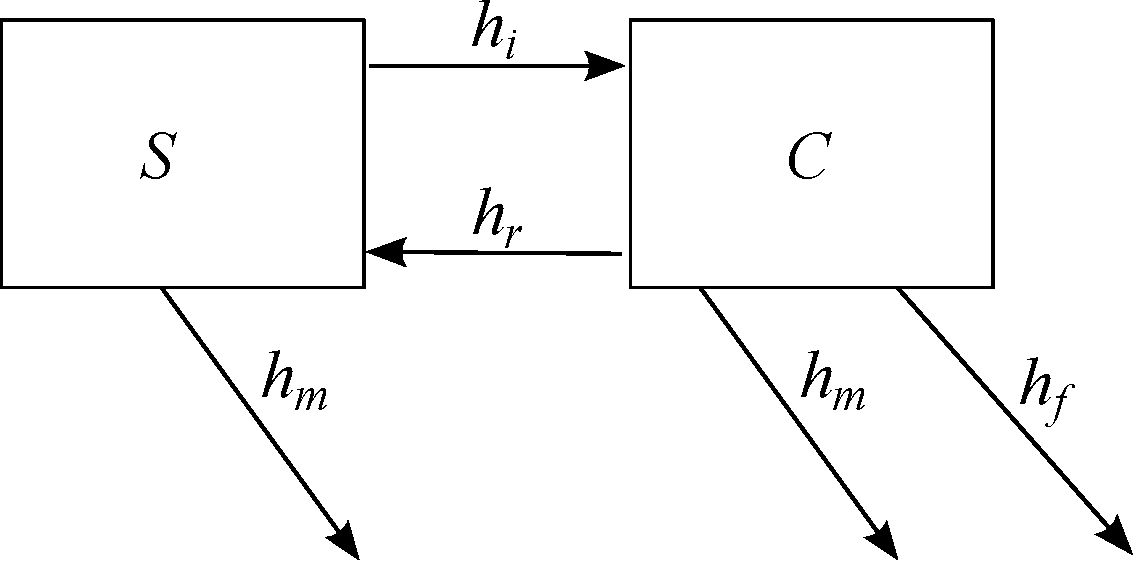
\includegraphics[width=5in]{SC.pdf}
            \caption{The two-compartment model of process for disease in a population, around which the metaregression framework is built. Compartment $S$ contains the population susceptible to the disease and compartment $C$ contains the population with the condition. Individuals move from $S$ to $C$ with incidence hazard $h_i$, and from $C$ to $S$ with remission hazard $h_r$. The susceptible population flows out of the system with without-condition mortality hazard $h_m$, and the with-condition population flows out of the system with with-condition mortality hazard $h_m+h_f$, where $h_f$ is the excess mortality hazard, representing quantitatively the increase in mortality for individuals with the condition.}
            \label{forward-sim-two-compartment}
        \end{center}
    \end{figure}

The precise mathematical representation of this model will be
elaborated on in great detail in
Chapter~\ref{forward-simulation}. Without going into details, it is
intuitive that there must be a relationship between
incidence, prevalence, remission, and with-condition mortality. The
data that has been gathered for each of these epidemiological
parameters should all be brought together in a theoretically grounded
process of data confrontation to produce a best estimate and plausible
uncertainty bounds for disease incidence and prevalence, if this is to
be used in YLD estimation. Through this grand synthesis of a
meta-analysis, I hope to produce the best possible estimates of
disease burden.


\section{History of generic disease modeling}

The line of research into disease modeling for descriptive
epidemiology has been accompanied by software implementations since
the 1990s.  The development and refinement of these computer codes
provides conveniently named milestones through the history of the
approach.  For example, DisMod I was software developed in the early
1990s to support analysis in the original Global Burden of Disease
Study.  Computing power has increased dramatically over the 20-year
period in which the DisMod family of generic disease modeling software
has evolved, and the aspiration of methods has expanded as well. We
now trace how the approach has evolved from a simple spreadsheet model
to a robust meta-regression framework.

The precursor to the first DisMod, the Harvard Incidence-Prevalence
(HIP) Model, was a spreadsheet implemented in Lotus 123.
\cite{Murray_Quantifying_1994} This model took as input a set of
instantaneous incidence, remission, and excess mortality rates for $5$
age groups, and produced estimates of disease prevalence and duration.
The model involved constructing a life table to simulate a cohort
exposed to a set of age-specific incidence, remission, case fatality
and background mortality hazards. At each year in the life table, the
model simulated a simple 3-compartment model to provide estimates of
the number susceptible, the number of cases and the number of deaths
to input into the life table for the next year.  It was used primarily
for three purposes: to find prevalence for conditions where incidence
is known and reasonable assumptions about remission and excess
mortality can be made; to find attributable deaths that were not
directly coded to a specific cause; and to find incidence for
conditions where prevalence is known.  The third use case required an
interactive procedure in the HIP model, since the input incidence was
unknown.

As is often the case in science, a very similar approach had been
developed previously by researchers at the International Institute
for Applied Systems Analysis in Austria in the 1970s.\cite{international_institute_for_applied_systems_analysis._estimation_1977} This work was
part of a broad program to develop a generic Healthcare System Model
to improve management and planning in the health sector. One component
of this model was a computer program to estimate prevalence from
incidence. That program evolved a population
exposed to age-specific incidences of disease and death through time.
Although it was designed specifically for terminal illness, it is
similar to the DisMod line of models in many ways. It was applied to
estimate the prevalence of malignant neoplasm in Austria, France and
Belgium.


Over the course of the first Global Burden of Disease Study, the HIP
Model evolved in DisMod
I.\cite{murray_global_1996}
This was formalized as a four compartment model, and corresponding
system of differential equations.  Like the HIP model, the input to
DisMod I consisted of instantaneous rates for incidence, remission,
and excess mortality, now specified for $9$ age groups.  In addition
to the three use cases from the HIP model, DisMod I was also used to
estimate the average duration of disabling sequelae, as a function of
age.  DisMod I was used iteratively by analysts working on the GBD 1990
study to identify a solution that matched the available data on
prevalence, incidence, remission, excess mortality and cause-specific
mortality.  DisMod I was used to address multiple challenges: mapping
from incidence data to prevalence and vice-versa; assessing the
consistency between incidence, prevalence and cause-specific mortality.

DisMod II moved from forward simulation into the realm of
optimization.  It provided more control over inputs, as well as a a
graphical user interface and comprehensive user manual, making it more
widely usable than previous iterations.\cite{Barendregt_Generic_2003}
In addition to accepting input of instantaneous rates for incidence,
remission, and excess mortality, DisMod II was also capable of using
age-specific prevalence and cause-specific mortality rates, as well as
incidence as a population rate, and duration when it is short (less
than one year).  It also provided an algorithmic method for data
confrontation, wherein the downhill simplex method was used to
minimize the weighted difference between the inputs and the output
predictions.  Although DisMod II included the step towards
optimization, it was not framed as a statistical likelihood estimation
and thus did not generate uncertainty intervals.  To put it another
way, there was not measurement model included, only the model relating
true population rates.

The generic disease modeling approach was distributed without cost by
the World Health Organization (WHO) through the DisMod II software. It
has been used widely in burden of disease studies over the last 10
years. These studies adopted the methodology of the global study, but
aimed to assess burden at a level of detail more relevant for national
policymakers. Nearly $45$ countries have undertaken national or
subnational burden of disease study, including studies in Mexico,
Chile, Colombia and
Mauritius.\cite{Lozano_Burden_1995,republica_de_colombia_ministerio_de_salud_carga_1994,concha_barrientos_carga_1996,Vos_Mauritius_1996}

Despite its wide application, DisMod II has not been without
criticisms.  One methodological concern that emerged from extensive
application of the model centered on the difficultly in producing
consistent estimates that exhibited face validity, for example age
patterns that increased monotonically as a function of age. Despite
strongly held prior beliefs on the part of domain experts, it was not
uncommon for the prediction to show oscillations as a function of age, due
to the contortions that DisMod II would subject rates to in order to
produce consistent estimates as close to the single rate type input
estimates as possible.

Another important challenge in the DisMod II work flow was the
production of single best estimates for at least three independent
rates to be used as input.  Systematic review often finds multiple
measurements of an age-specific rate, and only one could be the input to
DisMod II.  Transforming a large collection of measured values, often
for incommensurate age intervals, to a single best estimate of disease
prevalence was a difficult challenge in analysis that is a necessary
preprocessing step to do meta-analysis with DisMod II.

A third challenge with DisMod II was in producing robust estimates of
parameter uncertainty.  Although the system included a method to
propagate uncertainty in the input parameters through to the output
estimates, this was laborious and rarely used in practice.

Finally, although DisMod II excelled in providing consistent estimates
from the confrontation of inconsistent estimates of several disease
parameters for a single place and time, it was laborious on the part
of the data analyst to produce comparable estimates for a variety of
different places and times. In the Global Burden of Disease (GBD) 2010
Study, there are 21 geographic regions to produce estimates for, at
three different points in time, for males and females. Even an
analysis that is trivial for one region/time/sex becomes burdensome
when it must be replicated $126$ times.

For the GBD 2010 Study, we initiated a complete redevelopment of the
method, continuing the trend towards including more formal inferential
techniques into the estimation process.  The broad principle behind
this approach is what we call integrative systems modeling (ISM) and
can be characterized in two parts: a system dynamics model of process
and a statistical model of data, considered together, so that instead
of doing forward simulation, as is traditionally the case in system
dynamics modeling, the model is used to solve an inverse problem. This
approach is emerging as a powerful approach for developing models that
integrate all available data sources.  ISM, and its intellectual
history, is the topic of the the next section of this chapter.  On top
of the compartmental model initially conceived for the HIP model, we
have layered an age-standardizing negative binomial mixed effects
spline model, which is fit directly to the data extracted in
systematic review using Bayesian methods.  The details of this
approach constitute the bulk of the first half of this book.

%% \section{Integrative systems modeling}
%% \label{intro-ism}
%% A vast body of literature exists on compartmental modeling and its
%% wide applicability to modeling the dynamics of complex systems
%% \cite{Forrester_Principles_1968, Meadows_Thinking_2008,
%%   Bossel_Systems_2007}.  TK more words in the way of a general
%% introduction to this idea.  Something about Forrester's outsider
%% models of epi, something about the introductory textbook in
%% environmental science Consider a spherical cow, etc.

%% \subsection{Compartmental models in epidemiology}
%% In epidemiology, compartmental models are often constructed to
%% simulate infectious disease dynamics.\cite{Anderson_Infectious_1991}
%% The classic Susceptible-Infectious-Recovered (SIR) model evolves a
%% population through a Susceptible compartment to an Infected
%% compartment to a Recovered
%% compartment.\cite{Kermack_Contribution_1927} Infection dynamics are
%% captured by making the amount of mass that moves from the Susceptible
%% compartment to the Infected compartment dependent on the product of
%% the masses in the two compartments. This dependence implies that the
%% number of new infections will increase with the number of current
%% infections. Extensions of this basic model abound.\cite{Daley_Epidemic_2001,Brauer_Mathematical_2001} The transition
%% parameters in this class of compartmental models, for instance incidence and
%% remission in the case of the SIR model, are usually set
%% based on extracting point estimates of the parameters from literature
%% reviews. Uncertainty is usually assessed based on a sensitivity
%% analysis that solves the compartmental model for the range of
%% parameter estimates found in the literature (UCLA disease modeler who
%% started latin hypercube sampling) \cite{Nagelkerke_Modelling_2002,
%%   Brandeau_Screening_1993, Broutin_Impact_2010}.

%% In statistical analyses, this estimation approach would often be
%% considered insufficient. Instead, the analyst would attempt to find the
%% parameters that, for instance, maximized the likelihood of a set of
%% data samples of the parameter values. This statistical approach has
%% the advantage that uncertainty can be rigorously quantified and an
%% optimal estimate can be identified based on a transparent model.

%% Combining these approaches is currently the subject of basic research.
%% Statistical inference for mechanistic models can be found in full-information maximum likelihood via optimal filtering (FIMLOF) and ``plug-and-play'' inference methodologies. \cite{peterson_statistical_1980, he_plug_2010, breto_time_2009}

%% Advances in statistical modeling and computation have allowed
%% increasingly sophisticated models to be fit to data. These advances
%% have spawned a new modeling approach that seeks to provide more
%% reliable point estimates and estimates of uncertainty for parameters
%% in compartmental models. This new approach, integrative systems
%% modeling, connects a system dynamics model to a statistical model so
%% that parameters in the system can be estimated in a statistical
%% framework without sacrificing the structure provided by the dynamical
%% model.

%% The analyst building a statistical model has a rich vocabulary with
%% which to describe the data-generating process of interest. Data can
%% come from a range of distributions. Hierarchical data can be expressed
%% via random effects and smooth data through the correlation structure
%% of a covariance matrix. In the most mature forms of integrated systems
%% modeling, this rich vocabulary is made available for estimating
%% parameters in a compartmental model. My approach to the meta-regression of descriptive epidemiological data is a prime example of
%% connecting a sophisticated statistical model to a mechanistic model of disease progressing
%% through a population. The complexity of the statistical model and the
%% complexity of the underlying system dynamics model vary across
%% different applications.

%% \subsection{Compartmental models in pharmacokinetics}
%% The field of pharmacokinetics and pharmacodynamics (PK/PD) provides
%% some of the most sophisticated examples of connecting a statistical
%% model to a compartmental model.

%% Pharmacokinetics is the study of how drugs get absorbed and
%% distributed in the body. Pharmacodynamics is the study of the effect
%% of drugs on the body. Much of the content of these two fields overlap
%% so they are often studied together. Within PK/PD, the field of
%% population pharmacokinetics attempts to understand the sources of
%% variability in drug response among individuals
%% \cite{Yuh_Population_1994}. Because clinical trials provide data on
%% only a small subset of the target patient population and at small
%% sample sizes, it is often difficult to estimate variation among
%% individuals without imposing additional structure on the estimation
%% problem. In 1972, the field of population pharmacokinetics began in
%% earnest when nonlinear mixed effects modeling was proposed as a
%% solution to the limited clinical data
%% \cite{Sheiner_Modelling_1972}. The techniques that have emerged in
%% this field are mathematically identical to those necessary for estimation and prediction
%% in ISM meta-regression. Analysts in
%% population pharmacokinetics connect a random effects model of patients
%% within a study (the statistical model) to a compartmental model that
%% describes the process of a drug's absorption in the body (the system dynamics model).

%% Analogous to the advent of the DisMod software for simulating and
%% estimating generic disease models, many different software packages
%% have arisen to help conduct analyses in population
%% pharmacokinetics. NONMEM, which developed at UCSF, was one of the
%% first.\cite{Beal_NONMEM_2009} SAAM II, a computer tool for the
%% simulation, analysis and modeling of pharmacokinetic data, also allows
%% users to fit compartmental models of the drug response to clinical
%% data using the integrative systems modeling
%% approach.\cite{Barrett_SAAM_1998}

%% TK a little more about this, and its glories.





\section{Systematic review and meta-analysis}
TK History of systematic review and meta-analysis, from antiquity and
tracing its rise in prominanace in the medical sciences, togrether
with a justifi caion for its continuted practice, in terms of
summarizing the vast quantity of primary researech being
conducted. Distinguish systematic review from meta-analysis, following
the distinction made by PRISMA.

Wikipedia \url{http://en.wikipedia.org/wiki/Systematic_review}
\begin{quote} A systematic review is a literature review
  focused on a research question that tries to identify, appraise,
  select and synthesize all high quality research evidence relevant to
  that question. Systematic reviews of high-quality randomized
  controlled trials are crucial to evidence-based medicine.[1] An
  understanding of systematic reviews and how to implement them in
  practice is becoming mandatory for all professionals involved in the
  delivery of health care. Besides health interventions, systematic
  reviews may concern clinical tests, public health interventions,
  adverse effects, and economic evaluations.[2] Systematic reviews are
  not limited to medicine and are quite common in other sciences such
  as psychology, nursing, occupational therapy, physical therapy,
  educational research, sociology and business management.

A systematic review aims to provide an exhaustive summary of
literature relevant to a research question. The first step of a
systematic review is a thorough search of the literature for relevant
papers. The Methodology section of the review will list the databases
and citation indexes searched, such as Web of Science and PubMed, as
well as any individual journals. Next, the titles and the abstracts of
the identified articles are checked against pre-determined criteria
for eligibility and relevance. Each paper may be assigned an objective
assessment of methodological quality using the Jadad scale or similar
rating system.[3][4][5] Systematic reviews often, but not always, use
statistical techniques (meta-analysis) to combine results of the
eligible studies, or at least use scoring of the levels of evidence
depending on the methodology used. Systematic review is often applied
in the biomedical or healthcare context, but it can be applied in any
field of research. Groups like the Campbell Collaboration are
promoting the use of systematic reviews in policy-making beyond just
healthcare.

A systematic review uses an objective and transparent approach for
research synthesis, with the aim of minimizing bias. While many
systematic reviews are based on an explicit quantitative meta-analysis
of available data, there are also qualitative reviews which adhere to
the standards for gathering, analyzing and reporting evidence. The
EPPI-Centre has been influential in developing methods for combining
both qualitative and quantitative research in systematic reviews.[6]

Many healthcare journals now publish systematic reviews, but the
best-known[citation needed] source is The Cochrane Collaboration, a
group of over 28,000 specialists in health care who systematically
review randomised trials of the effects of prevention, treatments and
rehabilitation as well as health systems interventions. When
appropriate, they also include the results of other types of
research. Cochrane Reviews are published in The Cochrane Database of
Systematic Reviews section of The Cochrane Library. The 2010 impact
factor for The Cochrane Database of Systematic Reviews was 6.186, and
it was ranked 10th in the ``Medicine, General \& Internal'' category.[9]


\end{quote}

Wikipedia \url{http://en.wikipedia.org/wiki/Meta-analysis}
\begin{quote}
In statistics, a meta-analysis combines the results of several studies
that address a set of related research hypotheses. In its simplest
form, this is normally by identification of a common measure of effect
size, for which a weighted average might be the output of a
meta-analyses. Here the weighting might be related to sample sizes
within the individual studies. More generally there are other
differences between the studies that need to be allowed for, but the
general aim of a meta-analysis is to more powerfully estimate the true
``effect size'' as opposed to a smaller ``effect size'' derived in a
single study under a given single set of assumptions and conditions.

Meta-analyses are often, but not always, important components of a
systematic review procedure. Here it is convenient to follow the
terminology used by the Cochrane Collaboration,[1] and use
``meta-analysis'' to refer to statistical methods of combining
evidence, leaving other aspects of 'research synthesis' or 'evidence
synthesis', such as combining information from qualitative studies,
for the more general context of systematic reviews.

The term ``meta-analysis'' was coined by Gene V. Glass.[2]

The first meta-analysis was performed by Karl Pearson in 1904, in an
attempt to overcome the problem of reduced statistical power in
studies with small sample sizes; analyzing the results from a group of
studies can allow more accurate data analysis.[3][4] However, the
first meta-analysis of all conceptually identical experiments
concerning a particular research issue, and conducted by independent
researchers, has been identified as the 1940 book-length publication
Extra-sensory perception after sixty years, authored by Duke
University psychologists J. G. Pratt, J. B. Rhine, and associates.[5]
This encompassed a review of 145 reports on ESP experiments published
from 1882 to 1939, and included an estimate of the influence of
unpublished papers on the overall effect (the file-drawer
problem). Although meta-analysis is widely used in epidemiology and
evidence-based medicine today, a meta-analysis of a medical treatment
was not published until 1955. In the 1970s, more sophisticated
analytical techniques were introduced in educational research,
starting with the work of Gene V. Glass, Frank L. Schmidt and John
E. Hunter.

Gene V Glass was the first modern statistician to formalize the use of
meta-analysis, and is widely recognized as the modern founder of the
method. The online Oxford English Dictionary lists the first usage of
the term in the statistical sense as 1976 by Glass.[2][6] The
statistical theory surrounding meta-analysis was greatly advanced by
the work of Nambury S. Raju, Larry V. Hedges, Harris Cooper, Ingram
Olkin, John E. Hunter, Jacob Cohen, Thomas C. Chalmers, Robert
Rosenthal and Frank L. Schmidt.

\end{quote}

TK a discussion of the common cautions about comparing apples and
oranges in meta-analysis; quote from Cochrane Handbook
\url{http://www.cochrane-handbook.org/}.  But comparing apples and
oranges is exactly what we want to do sometimes, for example when
estimating population levels of nutritional risk factors, where
respondants are asked, ``how many servings of fresh fruits and
vegetables do you eat in a day?''

These concerns are not without grounds, however.  And the purpose of
this book is to develop a method for comparing the results of
descriptive epidemiological studies of disease prevalence, incidence,
remission, and mortality risk, which are focused on subpopulations
from varying age groups, sexes, regions, and time periods.  It is not
impossible, but it is not as easy as inverse variance weighting or
even random effects regression.

It is not without precedent, however.  The next section discusses the
legacy of ``generic disease modeling'', which my integrative approach
to descriptive epidemiological meta-analysis builds upon.




\part{Theory}

\section{Introduction and Background}
Integrative systems modeling builds on a larger tradition of system
dynamics modeling, a field that originated out of operations research
and industrial engineering.  System dynamics modeling is an method to
model the behavior of complex systems in terms of stocks, flows, and
feedback loops.  The intuition here is that \emph{stock variables}
quantify the amount of some material, or mass, (or population in
disease modeling) in a compartment at a particular moment in time,
while \emph{flow variables} quantify the amount of material moving
into, out of, or between compartments. The scope of applications for
system dynamics is enormous, and once you start thinking of systems in
this way it may seem that everything can be modeled as stocks and
flows.  This is true of many approaches to modeling, however.  The
scope of system dynamics modeling is vast, and the method is useful
across this vast scope. It has been applied to the study of complex
systems in economics, politics, environmental science, and a diverse
array of other fields.

Traditionally, there is a delineation separating system dynamics
modeling from statistical modeling in the following way: system
dynamics aims to develop a \emph{model of process}, while statistical
approaches focus on developing a \emph{model of data}. Models of
process attempt to explicitly represent the mechanisms behind some
system behavior (deterministically or stochastically), while models of
data often explicitly avoid requiring such mechanistic theories. The
advantage of using the system dynamics approach is that it can
incorporate structural assumptions about the system underlying the
data.  In most applications, however, the process models of system
dynamics and the data models of statistics remain separate.
Integrative systems modeling is an attempt to bring them together for
mutual benefit.

The field of system dynamics has grown out of the work of Jay Forrester, a
management professor at MIT with a background in science and
engineering, in the 1950s. Its first application was in explaining
employment cycles at the company's appliance plants [ref TK]. Managers
incorrectly assumed that cycles merely followed general, economic
cycles, but by developing a compartmental model of the system
underlying GE's appliance business, Forrester showed that the
employment cycles arose from feedback loops inherent to GE's internal
structure. This first application demonstrates a major theme in system
dynamics. In complex systems, determinants of system behavior
considered one-by-one may be insufficient to predict the behavior of
that system. The most important behavior in a complex system arises
out of interactions and feedback between processes in that system. In
the case of disease modeling, the information contained in modeling
the entire disease process of incidence, remission and mortality
can exceed the information contained in separate
analyses of each of these features of the disease epidemiology.

TK paragraph on forward simulation, which includes an simple example,
such as the growth of a population, or use of a renewable resource.

Pharmacokinetic and pharmacodynamic (PKPD) modeling, a subdiscipline
of pharmacology, developed an approach to compartmental modeling in
tandem with system dynamics modeling, largely independently.  However,
the mathematics behind the models of process are extremely
similar. The compartments in PKPD models represent organs and other
physical systems in the body, and stocks represent the quantities of
pharmacologically relevant compounds in these compartments.  The flows
model the process of the drug of interest being metabolized or
otherwise passing through the subject. Mathematically, these models
have precise parallels to the stock-and-flow models developed by
Forrester and colleagues for supply chain analysis. For instance, in
one experiment researchers used a system dynamics approach to model
glucose kinetics. They found that a three compartment model where two
compartments correspond to peripheral pools exchanging plasma at
different rates with a central pool best represented the physiology of
glucose kinetics in their test subjects (in this case, a sample of 7
sheep) [ref TK]. This particular model structure has arisen several
times in applications in pharmacokinetics. It is called the mammillary
model. In another experiment, researchers modeled the kinetics of FULL
NAME TK (EACA) in 6 human subjects. EACA is compound used to control
hemorrhage in patients with bleeding problems. The PKPD researchers
developed a multi-compartmental model, where EACA was infused in a
central compartment, distributed to fast and slow excreting peripheral
compartments, and cleared by two compartments, one representing renal
excretion of the drug, and another representing non-renal excretion
[ref TK]. In both of these examples, and in general practice in
pharmacokinetics, the compartmental model-of-process is connected to a
statistical model-of-data to go beyond forward simulation to develop
methods of statistical inference for compartmental models. This
connection is the central idea of integrative systems modeling, and
one will be developed in detail in later chapters.

There has increasing interest in applying system dynamics principles
to the modeling of health and health systems. Health systems are
particularly complex, with many actors and many feedback loops,
providing a large supply of systems modeling opportunities. The health
of a population is affected by a combination of biological, economic,
demographic, and political forces, and all of these spheres interact
in a unexpected ways. Since the 1970s, system dynamics models have
been applied to model these various forces in order to advance our
understanding of population health [refs TK]. The topics addressed
have included: disease epidemiology, substance abuse epidemiology,
patient flows in emergency care, health care capacity and delivery,
and interactions between health care and disease epidemiology. A
systems approach is often required, because isolating one part of a
public health problem and then addressing that may in fact adversely
affect other parts of the system. For instance, low tar/nicotine
cigarettes were developed to address one part of the burden of disease
caused by tobacco consumption, but consumer behavior was not taken
into account. Consumers tended to take longer, more frequent drags and
thus negated the benefit of the low tar/nicotine content [ref TK]. A
system approach would seek to simultaneously account for both the
effect of the tobacco product on the consumer and the consumer's
behavior. In the context of modeling the progression of a disease
through a population, a model that seems to describe infection
dynamics accurately may conflict with data on remission or
fatality. Only by modeling the three together can the analyst get the
most accurate and consistent estimates.

One area in which public health has a long tradition of compartmental
and system dynamics modeling is in infectious disease [ref Andersen
  and May, Heathecote, Sally Blower, others? see wikipedia
  compartmental models in epi page]. For example, the
Susceptible-Infected-Recovered compartmental model, which was discussed in
Section~\ref{TK}. This basic model has been extended in a variety of
ways in order to model increasingly more complex infectious disease
dynamics. For instance, in one study Nagelkerke and colleagues modeled
the impact of a range of interventions targeted at preventing
transmission of HIV/AIDS epidemics [ref]. They estimated impact using a
compartmental model where the population moved from an Uninfected
compartment to either treated or untreated Infected
compartments to an AIDS compartment to a Death from AIDS
compartment. 

Another example that makes an explicit connection between
epidemiological modeling and system dynamics is the recent work by
Kershenobich and colleagues, who applied a systems approach to
forecasting the prevalence of hepatitis C. They developed a
compartmental model tracking incidence, diagnosis and treatment of the
disease. For the incident population in the model, an individual moves
from an acute phase (which lasts for 6 months) to a chronic phase,
unless that individual is spontaneously cleared of the disease, is
treated and cured or dies. For the prevalent population in the model,
an individual moves from viraemic to non-viraemic, dies or gets
treated and cured. Separate models were also used to estimate the
mortality rate in different countries based on age, liver-related
deaths due to hepatitis C infection, and percent of the population
infected by infection drug users. Sensitivity analyses were conducted
by running the model for a number of input scenarios.  TK description
of what this model allowed the authors to do, and especially how hard
it would have been to do in any other way.

System dynamics has been applied not only to the study of disease
processes, but also the health system. Flaxman and colleagues
developed a stock-and-flow model to synthesize data on the
availability and distribution of insecticide treated bednets (ITNs)
and to predict the proportion of households who owned an ITN. This
analysis employed a Bayesian approach to estimate the parameters of
the compartmental model that describe the process of ITNs moving from
warehouses and other storage facilities into the household and
possibly getting discarded by the households or lost in the
distribution process.



TK connection to the references cited in this NIH RFP for systems modeling
\url{http://grants.nih.gov/grants/guide/pa-files/PAR-08-224.html}
\url{http://ajph.aphapublications.org/cgi/content/full/96/3/452}
\url{http://www.hpsig.com/images/f/f5/SD_background_for_public_health_%284.11.05%29.pdf}
\url{http://www.systemswiki.org/index.php?title=Health_System_Dynamics_References}
\url{http://www.chronicdisease.org/nacdd-initiatives/diabetes/professional-development/act-on-data/SDMResourceList.pdf}

TK review of all pubmed literature that has term system dynamics in
the keywords or something.

TK discussion of bednets model and analogy between this and population
PK approach.

\section{System dynamics model of disease in a population}
At the heart of the new generic disease model is a set of four
compartments representing my fundamental equations of population
health. The compartments represent the population susceptible to the
disease ($S$), the population with the condition ($C$), the population
dead due to other causes ($M$), and the population dead due to the
disease ($D$). The population moves between these boxes following the
arrows shown in the figure, transitioning from $S$ to $C$ with incidence
rate $i$, and from $C$ back to $S$ with remission rate $r$. The susceptible
population transitions into box $M$ with (without-condition) mortality
rate $m$, and the with-condition population transitions into box $M$ with
without-condition mortality rate $m$, and into by $D$ with ``excess
mortality rate'' $f$.

TK parallel between this fundamental model of disease and the demographer's
 basic demographic equation (aka the fundamental balancing equation)
 \url{http://books.google.com/books?id=CR-EXq4y8XAC&lpg=PA5&ots=_jJryixe4z&dq=%22basic%20demographic%20equation%22&pg=PA6#v=onepage&q=%22basic%20demographic%20equation%22&f=false}


\section{Compartmental Model}
\begin{figure}
\begin{center}
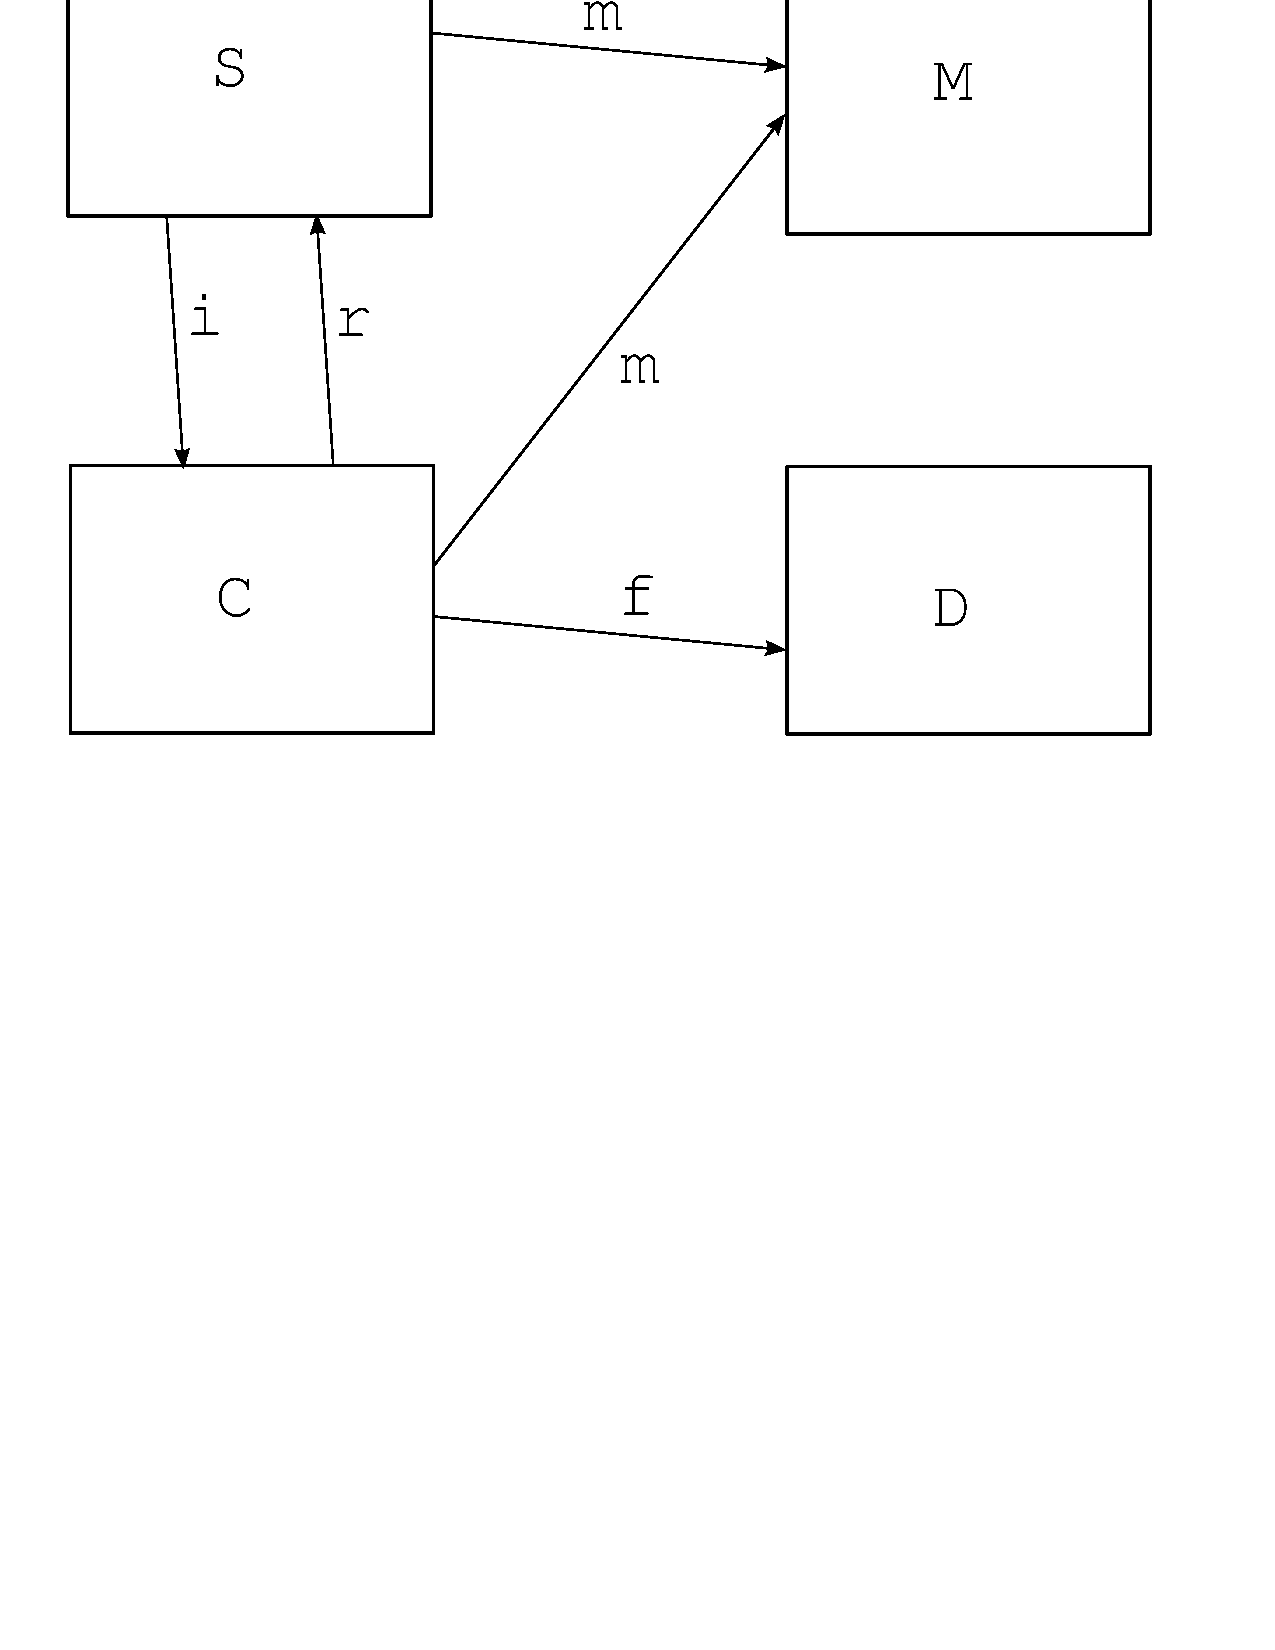
\includegraphics[width=\textwidth]{compartments.pdf}
\end{center}
\caption{TK updated caption; DisMod III uses a 4 compartment model to generate
  age-specific estimates of number without condition ($S$), number
  with condition ($C$), number of deaths not associated with the condition ($M$),
  number of deaths associated with the condition ($D$), incidence rate ($i$),
  remission rate ($r$), without-condition mortality rate ($m$), and
  excess mortality rate ($f$) (all shown in diagram); as well as
  prevalence ($p$), case duration ($X$), relative mortality risk ($RR$), all-cause mortality
  rate ($m_{all}$), and standardized mortality ratio ($SMR$).}
\label{fig:compartmental-model}
\end{figure}

TK Short discussion of what kind of epi study would be designed to
measure each of the important parts of this model. Comment that this
is not always what is available, and the bridge between what we know
and what we want to know will be developed in theory and practice in
several later sections of this book.

Conceptually, it is excess mortality $f$ that has proven hardest to
explain and to understand. This is because in most cases $f$ is a
latent variable, unobservable through most any epi study. Perhaps it
would be clearer to talk about the with-condition mortality rate,
which at least can be measured through a cohort study, and I think
will feel more familiar to the doctor or
epidemiologist. With-condition mortality is $m+f$, and the fact that
$M$ and $D$ are different boxes really is not that important when we
are doing generic disease modeling.

This 4 compartment model is really only a sketch of system dynamics
model I've used however, because it does not show age or time
information. In fact, there are large differences in disease
parameters such as incidence and prevalence as a function of age, and
it is essential for a model to take this into account.  Congenital
abnormalities all have a birth prevalence, while important diseases
such as dementia and Alzheimer's disease have much higher incidence
and prevalence at older ages. Furthermore the incidence and prevalence
of disease, as well as the remission rates and excess-mortality rates
change over time due to shifts in population, changes in prevention or
treatment, or changes in care. And the interdependence between these
factors is complex, but unignorable.  Today's 50-year-olds population
will be tomorrow's 51-year-olds, modulo migration and mortality as
least.

For these reasons, the 4 compartment model is more of a heuristic or
intuitive description of the system dynamics than a precise formal
definition.  A more accurate picture of the system dynamics model
shows the progression of the population as a function of time and age:

TK Time-age expanded version of the compartmental model above.

These figures are not up to the task of giving a full and precise
definition, however, and this is best expressed in terms of a system
of partial differential equations, describing the change in the size
of the compartments as a function of age and time. Although I have
made some simplifying assumptions for practical purposes, I believe
that it is worthwhile to start with the model that I would ideally
like to use, and then simplify it little by little so that it is
appropriately matched to the sparse data and/or the computational
resources available.

TK STOCHASTIC PDE GDM EQUATIONS, an embellishment of the following:

The full model is governed by the following system of partial
differential equations:
\begin{align*}
\frac{\partial S}{\partial (a+t)} &= -(i + m)S + rC,\\
\frac{\partial C}{\partial (a+t)} &= iS - (r + m + f)C,\\
\frac{\partial M}{\partial (a+t)} &= mS + mC,\\
\frac{\partial D}{\partial (a+t)} &= fC,
\end{align*}
where
\begin{align*}
S &= S(a,t) = \text{number without the condition of age $a$ at time $t$}\\
C &= C(a,t) = \text{number with the condition of age $a$ at
  time $t$}\\
M &= M(a,t) = \text{number dead not due to the condition (who would have been) of age $a$ at time
$t$}\\
D &= D(a,t) = \text{number dead due to the condition
  (who would have been) of age $a$ at time $t$}\\[.1in]
i &= i(a,t) = \text{incidence rate for people age $a$ at time $t$}\\
r &= r(a,t) = \text{remission rate for people age $a$ at time $t$}\\
m &= m(a,t) = \text{without-condition mortality rate for people age $a$ at
time $t$}\\
f &= f(a,t) = \text{excess mortality rate for people age $a$ at time
  $t$}
\end{align*}

\subsection{Simplifying assumptions}
\label{theory-forward_sim-compartmental_model-simplying_assumptions}

The first simplification which I have often used is to go from a
stochastic PDE to a deterministic PDE. This was done originally
because of the amount and quality of data available, as well as the
computation speed-up expected.  However, for certain data rich
settings, it may not be desirable. I suspect in the future generic
disease models will want to allow for stochastic PDEs as in the
equations above, and not be tethered by the simplifying assumptions
that I have made here. TK brief discussion of the assumptions inherent
in the deterministic model, and an investigation of how the stochastic
model could deal with these more robustly, for example deviation from
the Markovian assumption that people of age a have the same
with-condition mortality rate, regardless of whether they are a new
case or have had the condition for years. After this simplification,
the system of deterministic PDEs is the following:

\begin{align*}
\frac{\partial S}{\partial (a+t)} &= -(i + m)S + rC,\\
\frac{\partial C}{\partial (a+t)} &= iS - (r + m + f)C,\\
\frac{\partial M}{\partial (a+t)} &= mS + mC,\\
\frac{\partial D}{\partial (a+t)} &= fC,
\end{align*}

The second simplification comes from an assumption that the disease
parameters are not changing substantially with respect to time. TK
implications of simplifying assumptions on time stationarity, and
reduced equation that takes these assumptions into account.  DisMod
III follows the approach used previously, and assumes that the disease
parameters are not changing with time (i.e. the diseases is in endemic
equilibrium),
\[
\frac{\partial S}{\partial t}
=
\frac{\partial C}{\partial t}
=
\frac{\partial D}{\partial t}
=
\frac{\partial M}{\partial t}
=
\frac{\partial i}{\partial t}
=
\frac{\partial r}{\partial t}
=
\frac{\partial m}{\partial t}
=
\frac{\partial f}{\partial t}
=
0.
\]

This assumption on time derivatives is a big one, and deserves careful
assessment. In DisMod II, the default model also included the
assumption that the disease parameters did not change over time, but
an option allowed the model to incorporate assumptions of certain time
trends as well. I will return to the effects of this assumption in
section TK.

The next simplification is on the structure of the rates that dictate
the transitions between compartments (now as a function only of age).
By assuming that these rates are piecewise constant functions of age,
the system of partial differential equations has an explicit solution
for each interval on which the age is constant.

TK rewrite this lead in: Furthermore, DisMod III assumes that the rates are piecewise constant
functions of age, changing rate value only on a specified age mesh.  If
the age mesh is $\{a_0, a_1, \ldots, a_A\}$, then for any $a$ and $a'$
with $a_i \leq a, a' < a_{i+1}$,
\begin{align*}
i(a,t) &= i(a) = i(a')\\
r(a,t) &= r(a) = r(a')\\
m(a,t) &= m(a) = m(a')\\
f(a,t) &= f(a) = f(a')\\
\end{align*}

This permits me to solve the system of equations iteratively, starting
from the first interval, and proceeding interval by interval across
the entire age range. The solution for each age interval, after
assuming that TK FORMAL EQUATOIN OF ASSUMPTION takes the form of a
matrix exponential TK DISPLAY EQUATION.

These assumptions permit DisMod III to solve  explicitly for $S, C, D$
and $M$ iteratively.  The solution is conveniently expressed using the
matrix exponential:
\begin{equation}
\label{eq:ode-soln}
\begin{bmatrix}
S(a_{i+1})\\C(a_{i+1})\\M(a_{i+1})\\D(a_{i+1})
\end{bmatrix}
=
\exp\left(\begin{bmatrix}
-i(a_i)-m(a_i) & r(a_i)             & 0&0 \\
i(a_i)      & -r(a_i) -m(a_i) - f(a_i) & 0&0\\
m(a_i)      & m(a_i)             & 0&0 \\
0        & f(a_i)            & 0&0
\end{bmatrix}
(a_{i+1}-a_i)\right)
\begin{bmatrix}
S(a_i)\\C(a_i)\\M(a_i)\\D(a_i)
\end{bmatrix}
\end{equation}

There is another, related, simplification that is really more a matter
of computational convenience than mathematical simplification.  The
iterative solution to the difference equations above provides the
exact values on an age mesh $\{a_0, a_1, \ldots, a_I\}$, and this
appears in the inner-most loop of the computation, so it is a
significant time saving approximation to use linear interpolation to
fill in prevalence values between the points on the age mesh, instead
of using a more sophisticated differential equation solver to provides
a more precise solution to the system of ODEs. The effects of this
approximation can be minimized by choosing an age mesh appropriately,
and will be examined in more detail qualitatively later in the section
and quantatively in the Chapter TK on numerical algorithms.

Although the primary use of this model is for inference of model
parameters (sometimes called the ``inverse problem''), I can easily
apply it ``forwards'' to show how rates on incidence, remission, and
excess-mortality produce different prevalence curves. The next section
explores this forward simulation through a series of detailed
examples, to build up the reader's intuition around how consistency
forces interrelationships between prevalence, incidence, remission,
and mortality.


\section{Forward simulation examples}

When a generic disease model is initialized with all-cause mortality
data and nothing else, the initial values produce the following set of
consistent age patterns:

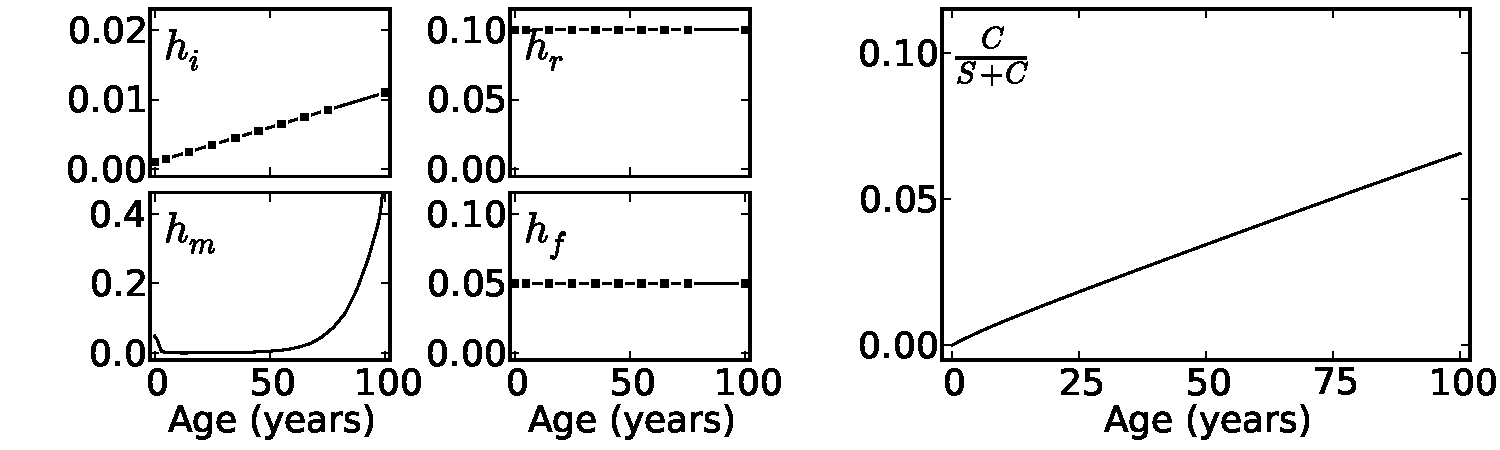
\includegraphics[width=\textwidth]{initial.png}

The next example shows that increasing the remission rate with
incidence and excess mortality unchanged (and all-cause mortality
unchanged as well) leads to a very different age pattern for
prevalence. It is also worth pointing out that since prevalence has
changed with excess mortality and all-cause mortality rates held
constant, the with-condition and background mortality rates have also
changed to maintain consistency.

\includegraphics[width=\textwidth]{more-remission.png}

By changing the incidence rate age pattern to be increasing as a
function of the square root age, I can demonstrate that very similar
prevalence rates are consistent with very different incidence and
remission rates.

\includegraphics[width=\textwidth]{increasing-incidence.png}

Although the prevalence age pattern is largely determined by the
remission, incidence, and mortality rates, the birth prevalence can
also change the shape dramatically.  Here are the results of the same
remission, incidence, and mortality rates as above, but with a birth
prevalence of 20\%.

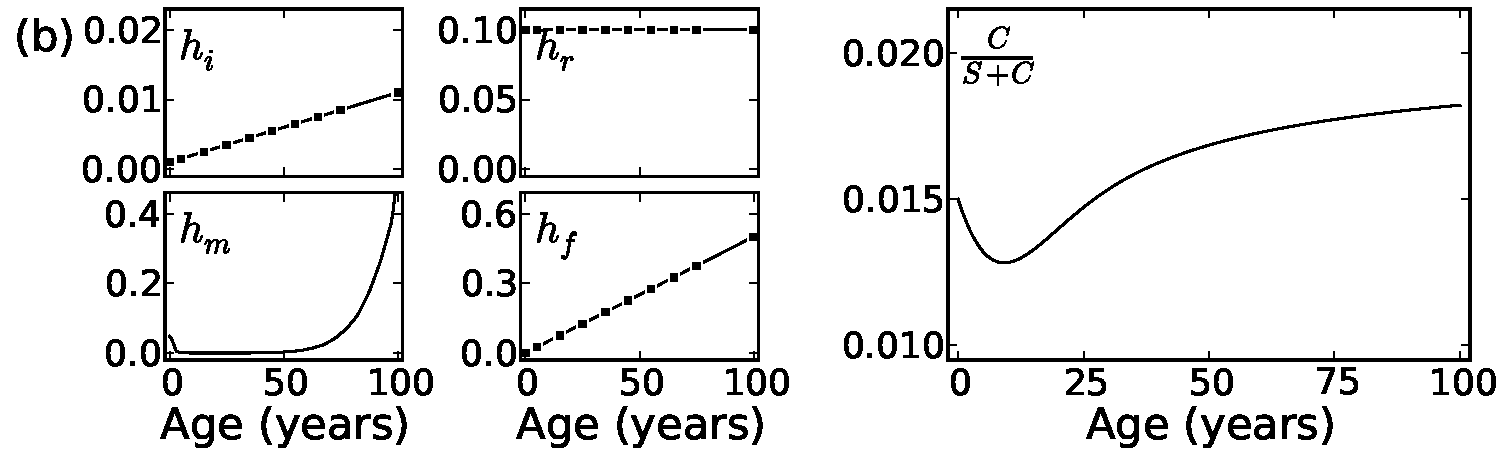
\includegraphics[width=\textwidth]{birth-prevalence.png}

An interesting, and perhaps unexpected feature of this set of
consistent rates above is that when prevalence levels start so high,
the levels remain high during the teenage years, where all-cause
mortality rates are quite low in this population (following the rates
for males in the North American High Income region in 2005), which
produces very low levels of background mortality for these age
groups. In other words, in order for the model to be consistent, it is
necessary to assume that the vast preponderance of teenage deaths are
due to this disease.

Finally, the excess mortality rate (which is the most difficult of the
rates to conceptualize, due to its unobservability) has an effect of
modulating the prevalence that is similar to the remission rate,
although not identical.  The final figure in this series shows the
results of choosing an excess mortality rate to have an age function
equal to ten times the all-cause mortality rate (which is to say a
standardized mortality rate of constant value eleven for all ages).

\includegraphics[width=\textwidth]{higher-smr.png}

The decreasing prevalence after age 65 is worthy of remarking
on. Although the incidence rate is increasing and the remission rate
remains unchanged, having a constant (albeit high) standardized
mortality ratio means that when all-cause mortality rises, the
with-condition mortality rises differentially with such magnitude that
the prevalence of the condition in older populations goes down.

To summarize, this series of figures has shown the intuitive and
less-than-intuitive way that the levels and age patterns of different
epidemiological parameters must be interrelated to satisfy the
fundamental equations of population health (when disease rates for
each age are changing negligibly slowly as a function of time).

The next series of figures continues to build familiarity with the
features of consistent disease modeling, by selecting age patterns for
certain rates based on toy models of a variety of diseases.  For
example, for a disorder like depression, for which there is primarily
incidence in early adulthood, high remission rate, and low excess
mortality, the consistency conditions produce a prevalence age pettern
that peaks at age 25: 

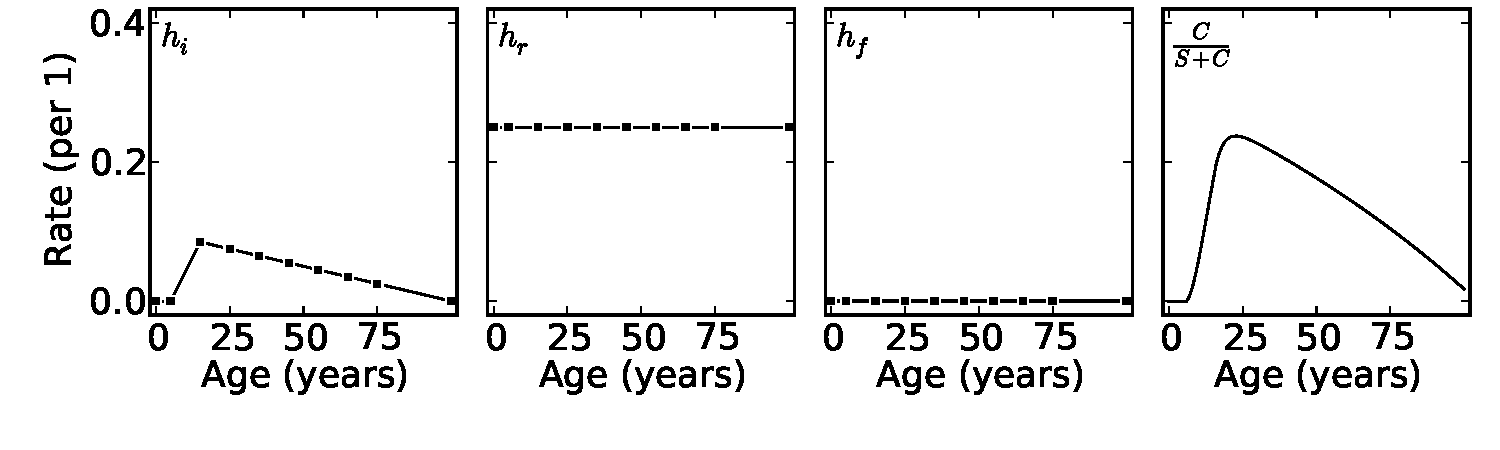
\includegraphics[width=\textwidth]{forward-sim-mental.png}

For a congenital disorder, like TK, with birth prevalence, no
incidence after birth, no remission, and substantial mortality, the
consistent prevalence age pattern is the following:

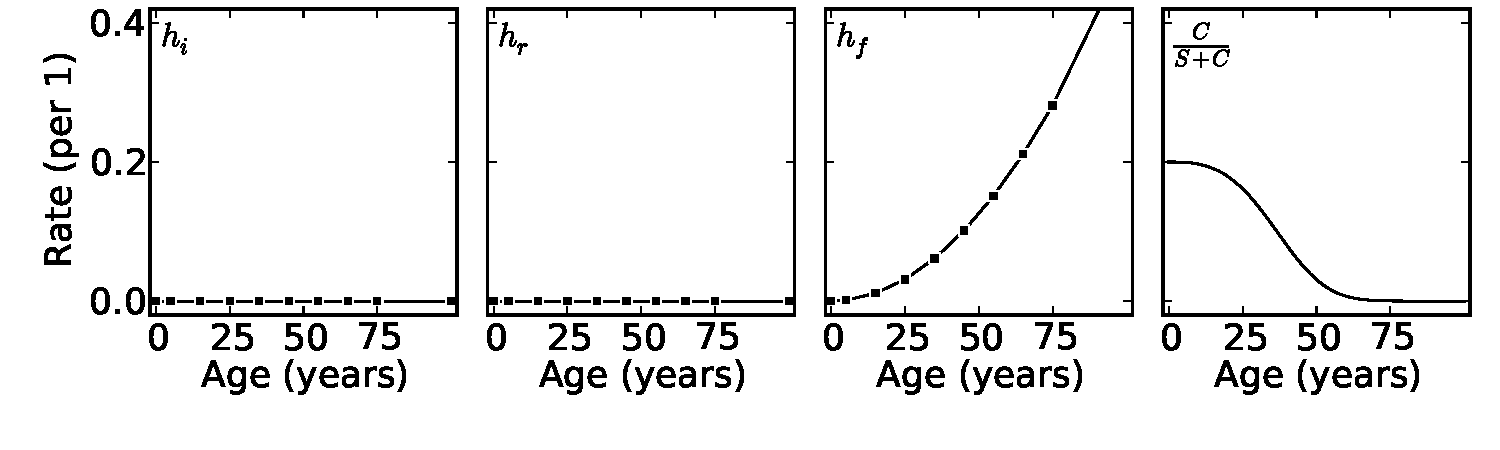
\includegraphics[width=\textwidth]{forward-sim-congenital.png}

For a disorder that affects the elderly, like TK, the consistent age
patterns for mortality, incidence, remission, and prevalence could
look like the following: 

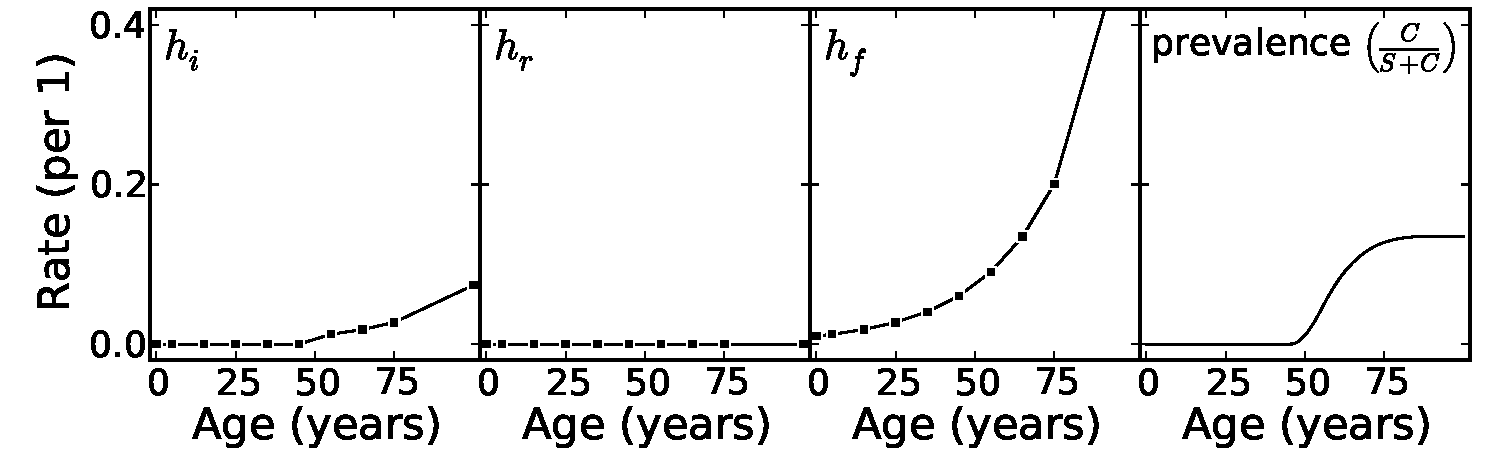
\includegraphics[width=\textwidth]{forward-sim-old_age.png}

And for a disorder related to the reproductive system, like TK, with
substantial excess mortality and incidence during ages 15-60, and
remission that increases substantially at age 55, the consistent age
patterns could look like the following: 

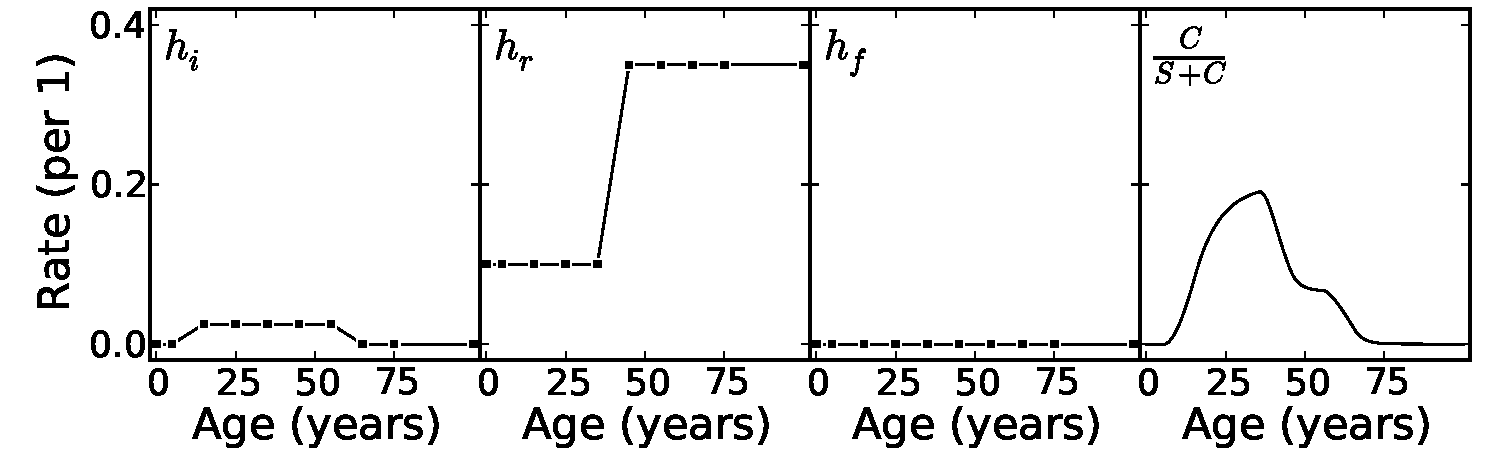
\includegraphics[width=\textwidth]{forward-sim-reproductive.png}

To conclude this series of plots, I've included an "incidence impulse
response" example, showing the prevalence produced to be consistent
with an incidence pattern that is only nonzero for a single age group:

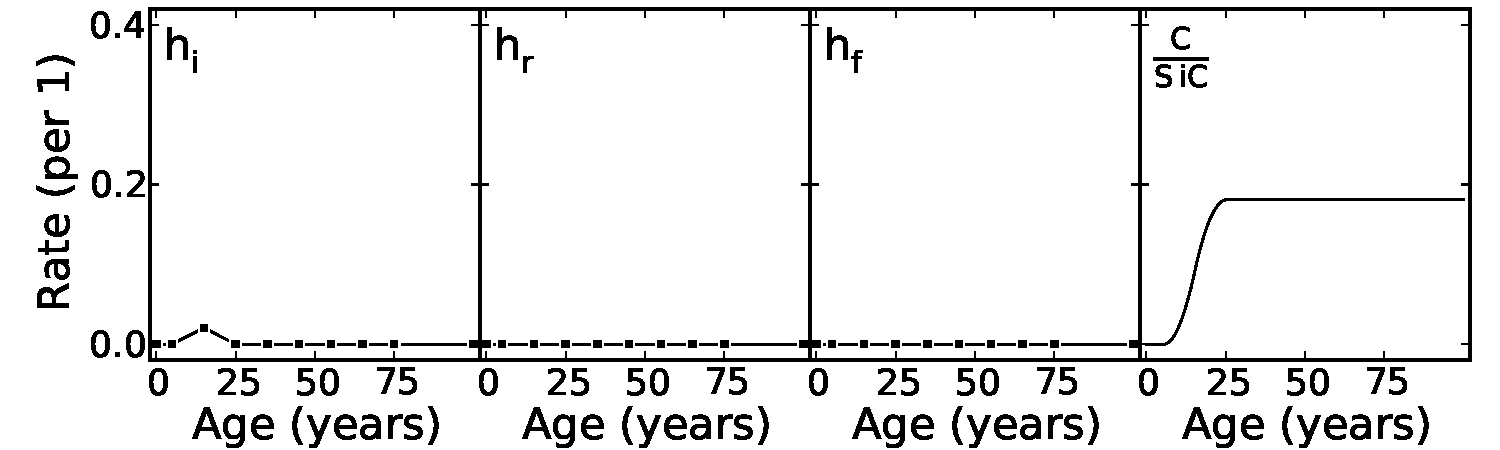
\includegraphics[width=\textwidth]{forward-sim-incidence_pulse.png}

This also provides a mechanism to investigate how wrong the estimates
may become when the assumption that rates are constant over time (for
a given age) is violated. This is the core of my simulation approach
to model validation, to which I will return in section TK.

TK The simulation study approach can be described in full detail here
as well, and can serve as justification for decisions described in the
next two chapters.

\section{What happens to prevalence when the disease incidence or remission or mortality is not constant over time?}

Certain important diseases such as diabetes are widely believed to
have substantial changes in incidence, remission, and mortality rates
over time.  What is the effect of the endemic equilibrium assumption
of the age-specific prevalence. TK plots comparing prevalence from a
synthetic cohort model to a period model using simulation data.

\chapter{Age pattern models}
\label{theory-age_pattern_model}
\chapterprecis{Abraham D. Flaxman}
The rate models of data in the previous chapter need several
extensions to be truly useful in descriptive epidemiological
metaregression.  The most important is representing the differences in
rates as a function of age.  In this chapter, I develop the
mathematical and statistical theory behind a model for age specificity
in prevalence rates as well as other epidemiological hazard functions,
such as incidence, remission, without-condition mortality, and
excess-mortality hazards.

Figure~\ref{ssas-mx_female_1990} shows age-specific all-cause
mortality rates for $5$-year age groups.  These mortality estimates are
for females in Southern sub-Saharan Africa in 1990.  A striking
feature of this plot is the range of variation in mortality levels as
a function of age.  They vary by $850$-fold between the minimum
in the $10$- to $14$-year-olds and the maximum at the oldest
ages. Epidemiological rates also vary among regions, times, and
sexes.  A figure like figure~\ref{ssas-mx_female_1990} for the Asia Pacific,
high income, region in 1990 would look very different, as
would the Southern sub-Saharan Africa region in 2010. However,
systematic variation as a function of \emph{age} is often the largest
source of variation by orders of magnitude, and furthermore, this
variation is often distinctly nonlinear.

\begin{figure}[h]
\begin{center}
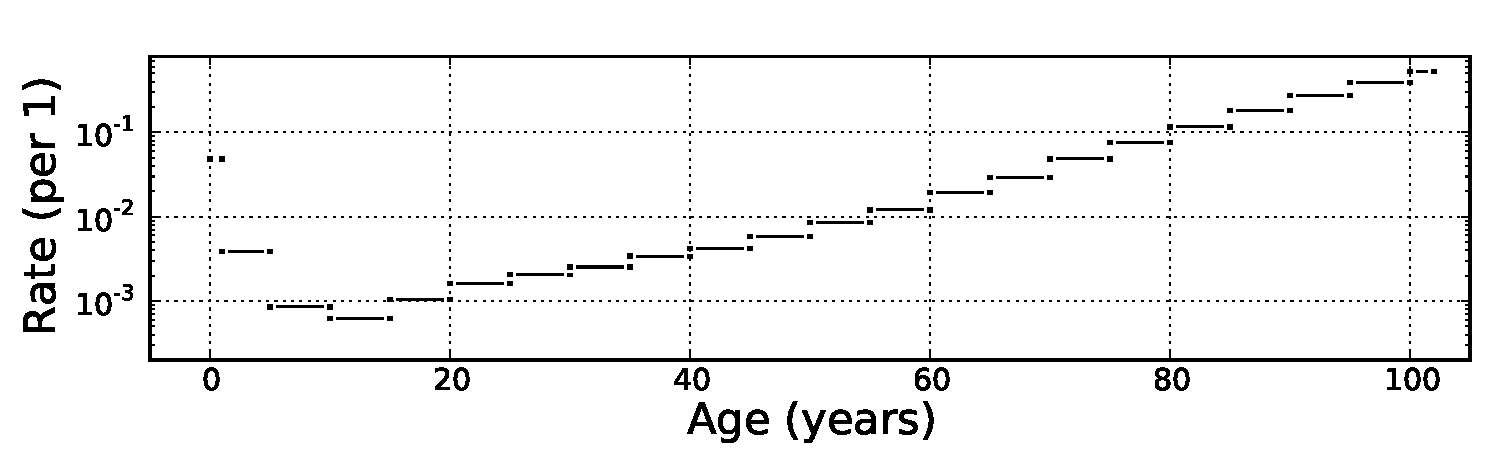
\includegraphics[width=\textwidth]{ssas-mx_female_1990.pdf}
\caption[All-cause mortality as a function of age.]{All-cause mortality for
  females in the Southern sub-Saharan Africa
  region in 1990 as a function of age shows the range of
  variation in age-specific rates.  All-cause mortality is as low as $6$ per
  $10,000$ PY at age $10$ but rises above $5000$ per $10,000$ PY at age $100$.}
\label{ssas-mx_female_1990}
\end{center}
\end{figure}

The approach that I have taken for modeling age-specific hazards draws
on the mathematical theory of spline interpolation and on the
statistical theory of penalized spline regression.  It is developed in
full detail in this chapter.


\section{Definition of spline models}
\label{spline_models}
For my purposes, a spline model can be any piecewise polynomial
function.  Often I will require this function to be continuous, but
not always.  This is a departure from the conventions of statistical
spline modeling, which focuses on continuous and continuously
differentiable splines.\cite{hastie_elements_2009,wahba_spline_1990}

I represent a spline model for an age-specific hazard $h(a)$ by a set
of knots $a_1,\dots,a_{K}$ and a set of piecewise polynomial basis
functions $\{p_1,\ldots,p_{K'}\}$.  Each knot has a corresponding
basis function, and for higher-order splines, there may be additional
basis functions as well, so $K \leq K'$.  The model then has $K'$
parameters, $\gamma_1,\ldots,\gamma_{K'}$, and takes the form
\[
h(a) = \sum_{k=1}^{K'} \gamma_k p_k(a).
\]

The mathematical definition of the model is straightforward, but the
detail of selecting the piecewise polynomials remains to be developed.
This is where the spirit of spline modeling lies. The knots $a_1,
\dots, a_{K}$ partition the age range into intervals. If I make each
piecewise polynomial $p_k(a)$ equal to $1$ on its interval (i.e., when
$a_k \leq a < a_{k+1}$) and $0$ otherwise, this yields a piecewise
constant spline model.  This is an important specialization, the
simplest of my spline models.  Using the notation $\1[a_k \leq a <
  a_{k+1}]$ to denote the function
\[f(a)
= \begin{cases}1,&\quad\text{if }a_k \leq a <
  a_{k+1};\\0,&\quad\text{otherwise;}\end{cases}
\]
 and the convention
that $a_{K+1} = \infty$, I can write out the piecewise constant spline
model as
\[
h(a) = \sum_{k=1}^K \gamma_k \1[a_k \leq a < a_{k+1}].
\]

By taking the piecewise polynomial corresponding to each knot as $0$
before its knot and a linearly increasing function after, the model
specializes to a piecewise linear spline model, a continuous
function that has a constant derivative at all nonknots.  By adding
an additional basis function that is not associated with a knot, this
piecewise linear spline model becomes a flexible approximation for any
nonlinear function and is the main form I have used in representing
age-specific hazards in the work to come.  I can write out the
piecewise constant specialization of the spline model as
\[
h(a) = \gamma_0 + \sum_{k=1}^K \gamma_k a \1[a \geq a_k].
\]

I find that in applications of this model it is useful to represent
the piecewise linear spline in an alternative basis, where the model
parameter $\gamma_k$ represents the values of $h(a_k)$ instead of the
change in the slope at this point.  This yields a more complicated set
of basis functions, but it is not necessary to write out the basis
functions explicitly.


Figure~\ref{splines_fig} shows the results of fitting spline models
for age-specific hazards to simulated data to minimize the sum of the
square differences between the predicted and observed values.  When
the piecewise constant model is fitted, it produces an age-specific
hazard function consisting of a series of horizontal (constant) lines
in each of the intervals between knots.  Interval $k$ has
$\gamma_k$ equal to the mean value of the simulated data between knots
$a_k$ and $a_{k+1}$, which is quite a sensible choice.

A more favorable and flexible fit to the data is achieved by the
piecewise linear spline model, which produces a continuous function
of age as its prediction. In many cases, a piecewise linear fit of
this type is sufficient to capture the nonlinearity in the data, and
this will be the typical model for epidemiological rates in the second
half of this book.  It is possible to go further along this path of
smoothing, however, and splines that have continuous derivatives and
even continuous second derivatives are popular alternatives, achievable
by simply choosing different piecewise polynomials for the basis
functions.


\begin{figure}[h]
\begin{center}
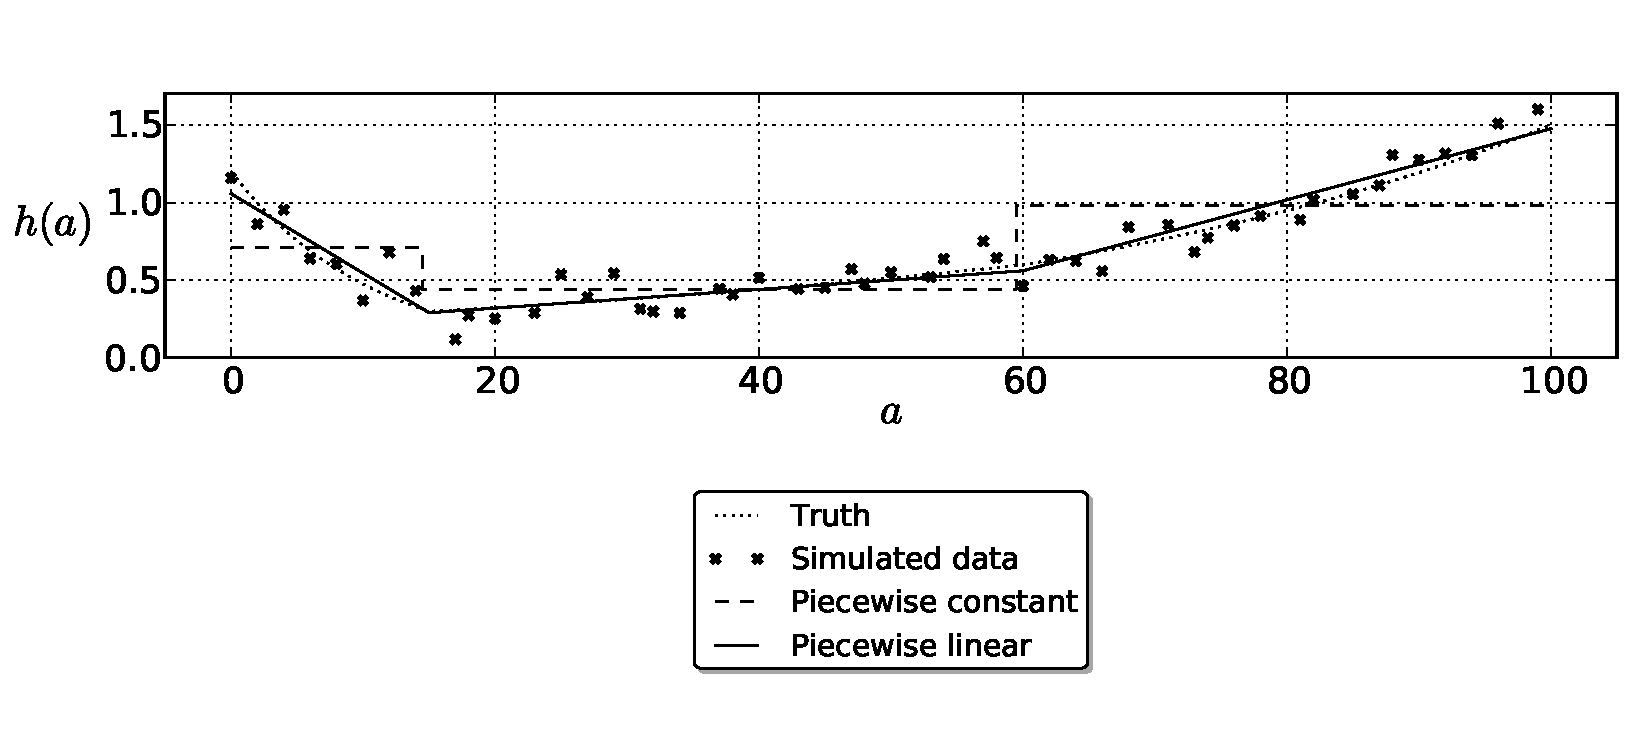
\includegraphics[width=\textwidth]{splines-fig.pdf}
\caption[Spline interpolation of simulated data.]{Spline interpolation
  of simulated data. The true age-specific
  rate is piecewise log-linear, so none of the splines can represent
  it perfectly. The true age-specific rate and the models all have
  knot set $\{0, 15, 60, 100\}$.}
\label{splines_fig}
\end{center}
\end{figure}


\section{Choosing knots}

To this point, I have taken as given the number and location of the
knots in the spline model. However, selecting the number and location
of the knots is an important task, and when working with sparse and
noisy data, this can influence the model results
substantially.

When data are abundant and age patterns are clear, models will not be
very sensitive to the choice of knots.  When data are not abundant, or
when the age patterns are not clear from the data, however, knot
selection is an important part of the modeling process.  In this
setting, knot locations should be chosen a priori, based on expert
knowledge about the disease being modeled. For example, in a recent
study looking at global trends in mean systolic blood pressure as a
function of age, the modelers chose to use a cubic regression spline
with knots located at ages $30$ and $60$.\cite{danaei_national_2011} These
choices reflect the expectation, based on literature and prior
knowledge, that the behavior of mean systolic blood pressure as a
function of age would be distinct in these intervals due to low blood
pressure in young adults and to survivor effects in elderly populations.

Although this approach of using expert knowledge to inform the choice of the number
and location of knots is practical and allows for users to
determine critical features of the model, it is certainly not the only
approach. Much literature is devoted to the choice of knot locations
and the number of knots.
An important direction for future work is to remove the reliance on
expert knowledge to inform knot selection.  This could proceed
through model selection or model averaging of models with a variety of
knot locations, \cite{raftery_bayesian_1997} through
techniques developed in the adaptive regression spline literature,
\cite{friedman_multivariate_1991} or by leaving spline models altogether and using Gaussian
processes or some similar nonparametric model for the age pattern.
\cite{rasmussen_gaussian_2006,diggle_model-based_2010}

\section{Penalized spline models}
One approach to address the challenge of knot selection is to include
more knots in the model and then also include a penalty function to
discourage the model from using the additional knots when the data
do not call for them.  This penalized spline model can be formulated in a
Bayesian framework by introducing a prior that represents the belief that, in
the absence of evidence, the age pattern does not vary.
Mathematically, this takes the form of a penalty on the root mean
square of the derivative of the age-specific rate $h(a)$:
\[
\left[\int _{a=a_1} ^{a_K} \| h'(a) \|^2 \d w(a)\right]^{1/2} \sim N(0, \sigma^2).
\]
This introduces an additional model parameter, $\sigma$, which can be
viewed as a hyperprior and controls the amount of smoothing that the
penalty creates.

For the piecewise linear penalized splines that will be used most
frequently in the second half of this book, the derivative of $h$ is
constant between knots, so, with equal weighting for smoothing at all
ages, the integral above simplifies to the following:
\begin{align*}
\int _{a=a_1} ^{a_K} \| h'(a) \|^2 \d a
& = \sum_{k=1} ^{K-1} \left[\frac{h(a_{k+1}) - h(a_k)}{a_{k+1}-a_k}\right]^2 \frac{a_{k+1}-a_k}{a_K - a_1}\\
&= \sum_{k=1} ^{K-1} \frac{\left[h(a_{k+1}) - h(a_k)\right]^2}{(a_{k+1}-a_k)(a_K - a_1)}.
\end{align*}
Figure~\ref{smoothing-splines} shows the effect of increasing the
smoothing parameter $\sigma$ when many more knots than necessary have been included in the model.

\begin{figure}[h]
\begin{center}
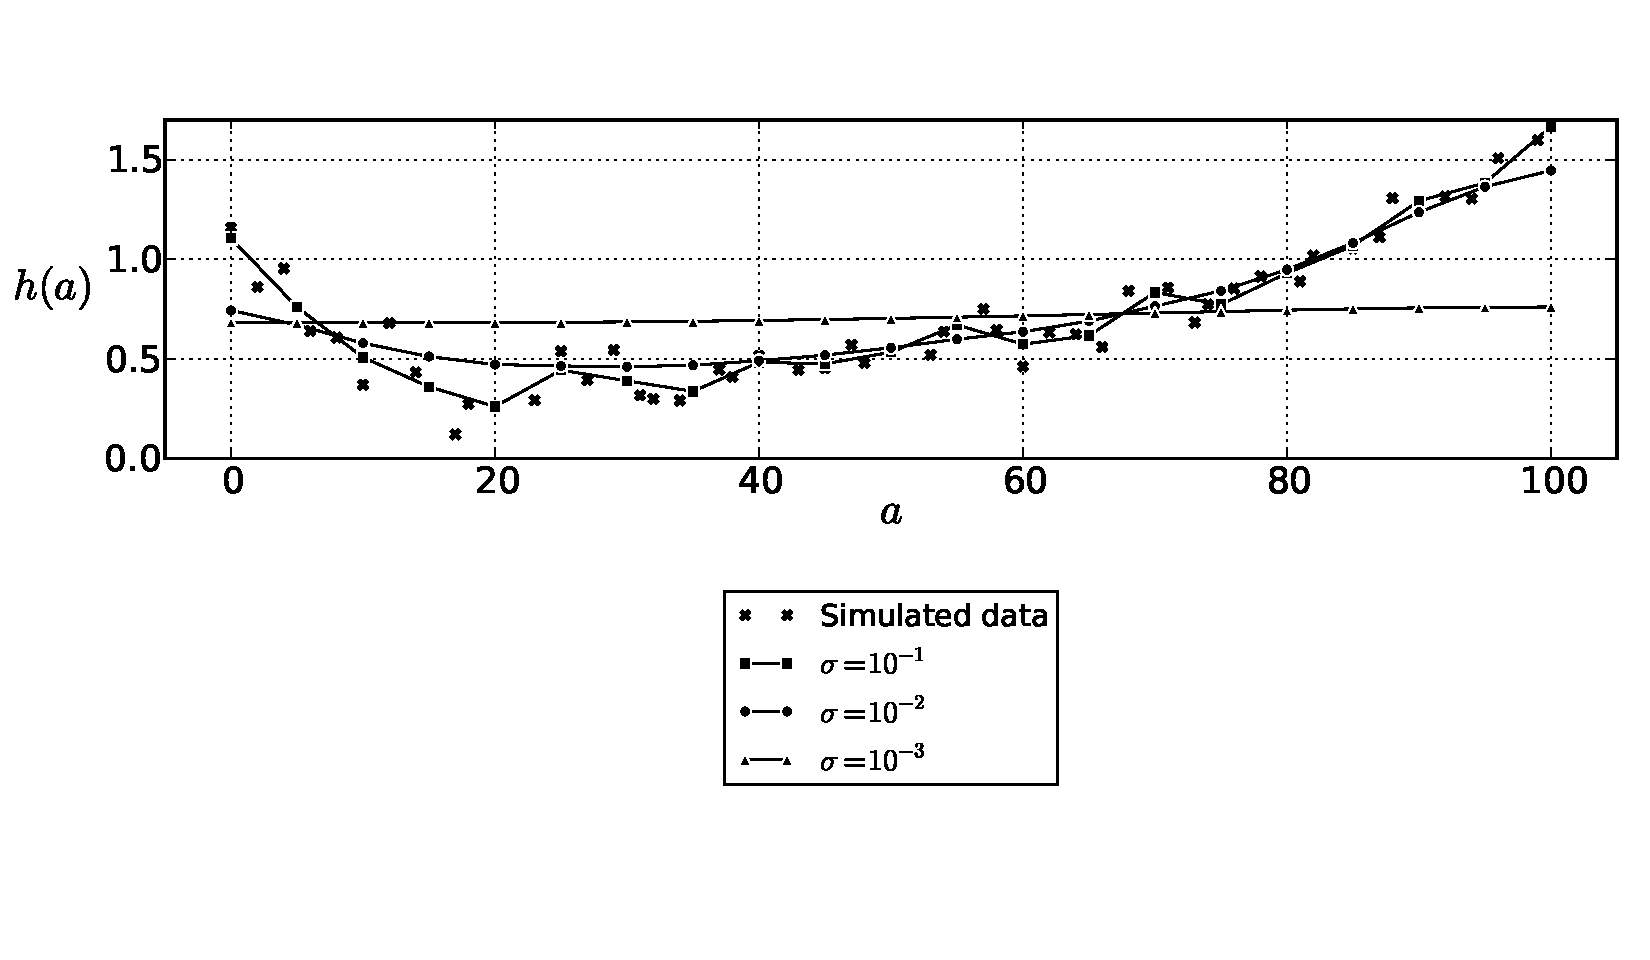
\includegraphics[width=\textwidth]{smoothing-splines.pdf}
\caption[Penalized splines with a carefully chosen smoothing
  parameter.]{Penalized splines with a carefully chosen smoothing parameter
  $\sigma$ provide a solution to the challenge of knot selection in
  spline modeling.  Without smoothing, including many knots leads to
  estimates that are overly uncertain and wiggly.  Smoothing, in the
  form of a quadratic penalty on the derivative of the age pattern,
  allows many knots to be included.  But too much smoothing, for
  example, $\sigma=10^{-3}$ in this case, results in a model that does
  not reflect true patterns in the data.}
\label{smoothing-splines}
\end{center}
\end{figure}


\section{Augmenting the spline model}
There are a few ways to augment the spline model that are useful when
modeling age-specific rates. Since the epidemiological rates I have modeled
are always nonnegative, I have parametrized the spline in
terms of the log of the knot values, so that $h(a)$ is a piecewise
linear spline model with knots $a_1,\ldots,a_K$, and
\[
h(a_k) = e^{\gamma_k}.
\]
To fit the model in a Bayesian framework, I have defaulted to
giving these $\gamma_i$'s ``weakly informative'' priors,
\[
\gamma_i \sim \Normal\left(0, 10^2\right).
\]
This has very little effect on the posterior distribution but makes
the prior ``proper'' and also helps with algorithm convergence in
some instances. Where relevant expert knowledge is
available, I can replace this with a more informative prior (this idea
is elaborated in chapter~\ref{theory-expert_priors}).

Finally, to deal with the order-of-magnitude differences of
age-specific rates, I have applied the smoothing penalty to the
logarithm of the rate rather than to the rate itself.  This creates an additional
complication, however, because the informative priors often say that
rates are $0$ for certain ages.  To avoid the ill effects of
smoothing when the rate contains values of $0$, I have
rounded up any $\gamma_i$ values that are below $10$ times the mean
rate.  The approach is operationalized as a penalty term in the prior:
\[
\widetilde{\|h'\|} = \sqrt{\sum_{k=1}^{K-1}
\frac{\left[\max(\gamma_k, \gamma_{\min})
-
\max(\gamma_{k+1}, \gamma_{\min})\right]^2
}{(a_{k+1}-a_k)(a_K-a_1)}} \sim \Normal(0, \sigma^2),
\]
where
\[
\gamma_{\min} = \log\left[\bigg(\sum_{i=0}^K e^{\gamma_i}/10\bigg)
/ K\right].
\]

Taken all together then, the model for an age-specific hazard function
that will be used in this book is
\begin{align*}
h(a) &= \sum_{k=1}^{K-1} \1[a_k \leq a < a_{k+1}]
\left( \frac{a-a_k}    {a_{k+1}-a_k} e^{\gamma_k}
     + \frac{a_{k+1}-a}{a_{k+1}-a_k} e^{\gamma_{k+1}}\right),\\
\gamma_k &\sim \Normal\left(0, 10^2\right),\\
\widetilde{\|h'\|} &\sim \Normal(0, \sigma^2).\\
\end{align*}
The value of $\sigma$ is a model parameter that will receive a very
informative hyperprior; for example, ``slightly smooth'' is
represented by $\sigma=0.1$.




\chapter{Expert priors on age patterns}
\label{theory-expert_priors}
\chapterprecis{Abraham D. Flaxman}

When dealing with sparse and noisy data, it is sometimes necessary to
include additional expert knowledge on the age pattern of
epidemiological rates.  For example, data sparsity can take the form
of a lack of information about age-specific hazards of disease in children.  In
diseases that are rare or nonexistent in children, the fact that incidence is
effectively $0$ before a certain age is known by disease experts but
not represented in the data collected by systematic review.

A benefit of the Bayesian methods that will be used to fit these
models is the conceptual and practical simplicity of adding additional
information to the age pattern model.  This is implemented by choosing
a more informative prior distribution.  For example, if the
epidemiology of a disease is such that the incidence level must be
$0$ before age $a_k$, this can be incorporated by replacing the
weakly informative prior by the conditional probability density with
this constraint included.

Three classes of additional information will come up
frequently in the applications later in this book: level bound priors,
level value priors, and monotonicity priors. This section describes
how each can be implemented as an informative prior on the age pattern
model.


\section{Priors on level}

Informative priors on the level of the age pattern seem simple at
first but may have unintended effects.  A prior on the level value for
certain ages says precisely that the age pattern should have that
value for those ages.  For example, figure~\ref{level-value-priors}
shows the effects of adding a prior where the age-specific hazard function takes values extremely
close to $0.1$, $0.5$, or $1.0$ from age $0$ to $15$.


\begin{figure}[h]
\begin{center}
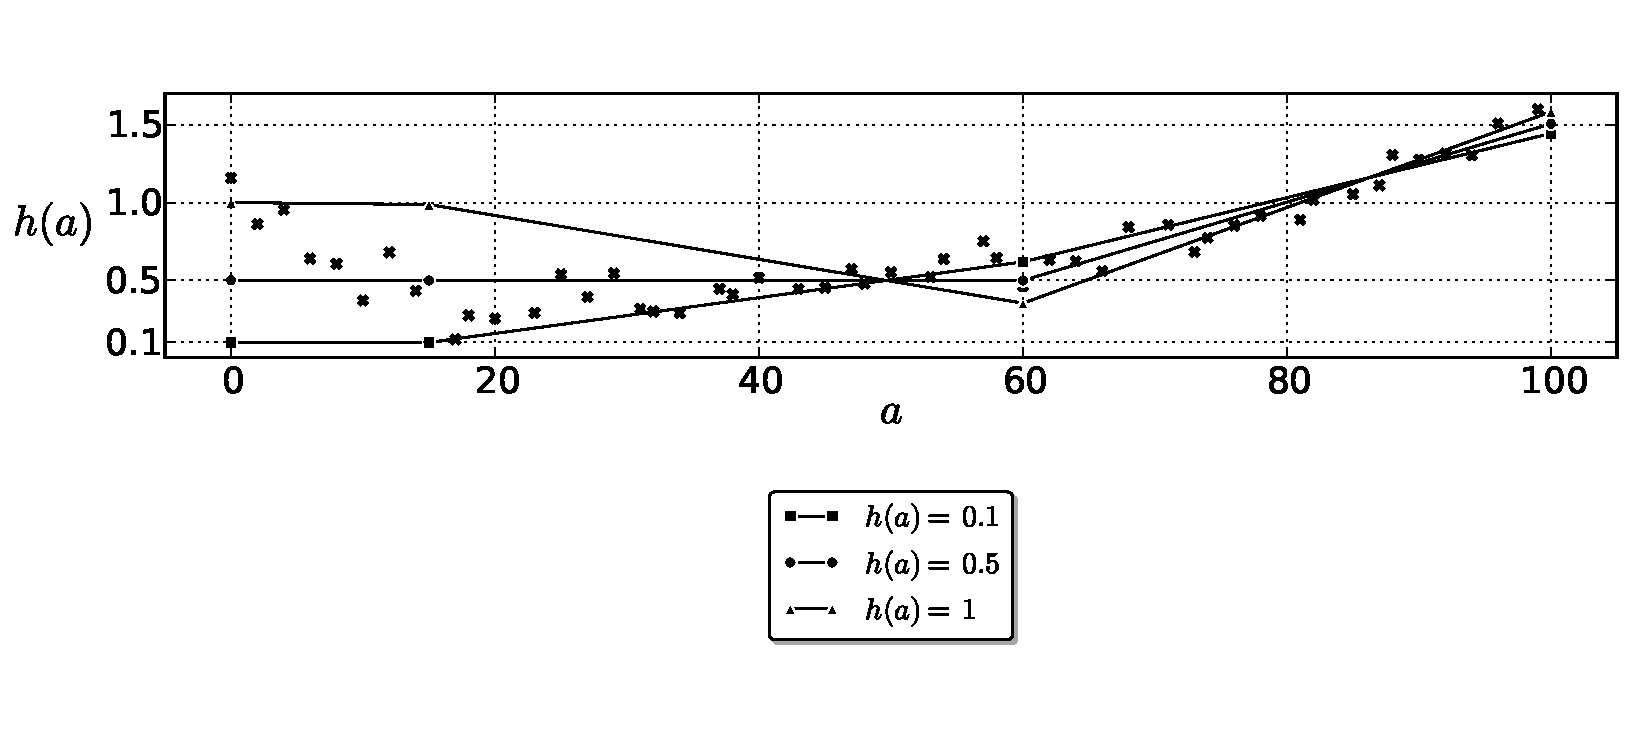
\includegraphics[width=\textwidth]{level_value-smoothing-splines.pdf}
\caption[An informative prior on the level of $h(a)$.]{An informative
  prior on the level of $h(a)$ for interval $0 \leq a <
  15$ changes the estimated rate dramatically for $a$ between $20$ and
  $60$ and even leads to different estimates for $a = 100$.  The more
  data available, the more knots in the model; the lesser the
  smoothing penalty, the less this level value assumption will affect
  the estimates for ages outside the interval, however.  }
\label{level-value-priors}
\end{center}
\end{figure}



These priors are implemented as ``hard-soft constraints.''  For a
value $v$ on age range $(a_0,a_1)$, the value of the spline model is
replaced with the level value for the age range (which I call a hard
constraint), and the prior density on the spline is augmented with a
penalty term for the offset log difference between the level value of
the unconstrained spline and $v$ (which I call a soft constraint). The
offset log difference penalty has the form
\[
\log\left(h(a)+\e)\right) \sim
 \Normal\left(\log\left(v + \e\right), \sigma^2\right),
\]
where $h(a)$ is the age-specific hazard function, $\e = 10^{-6}$ is the
offset to avoid taking the log of $0$, and $\sigma = 0.01$ is the
magnitude of the penalty.  In Bayesian terms, this encodes the belief
that the spline is expected to be within $1$\% of the expert level
value, provided the level value is not too close to $0$.

A similar sort of expert knowledge on the plausible bounds on
level is also useful, both in modeling noisy data and in increasing
the numerical stability of estimation algorithms. Again, however, the
implications of such a prior can be unexpected.
Figure~\ref{level-bounds-priors} shows the effects of three different
upper bounds on the spline estimation from the same data set as the
previous figure.

\begin{figure}[h]
\begin{center}
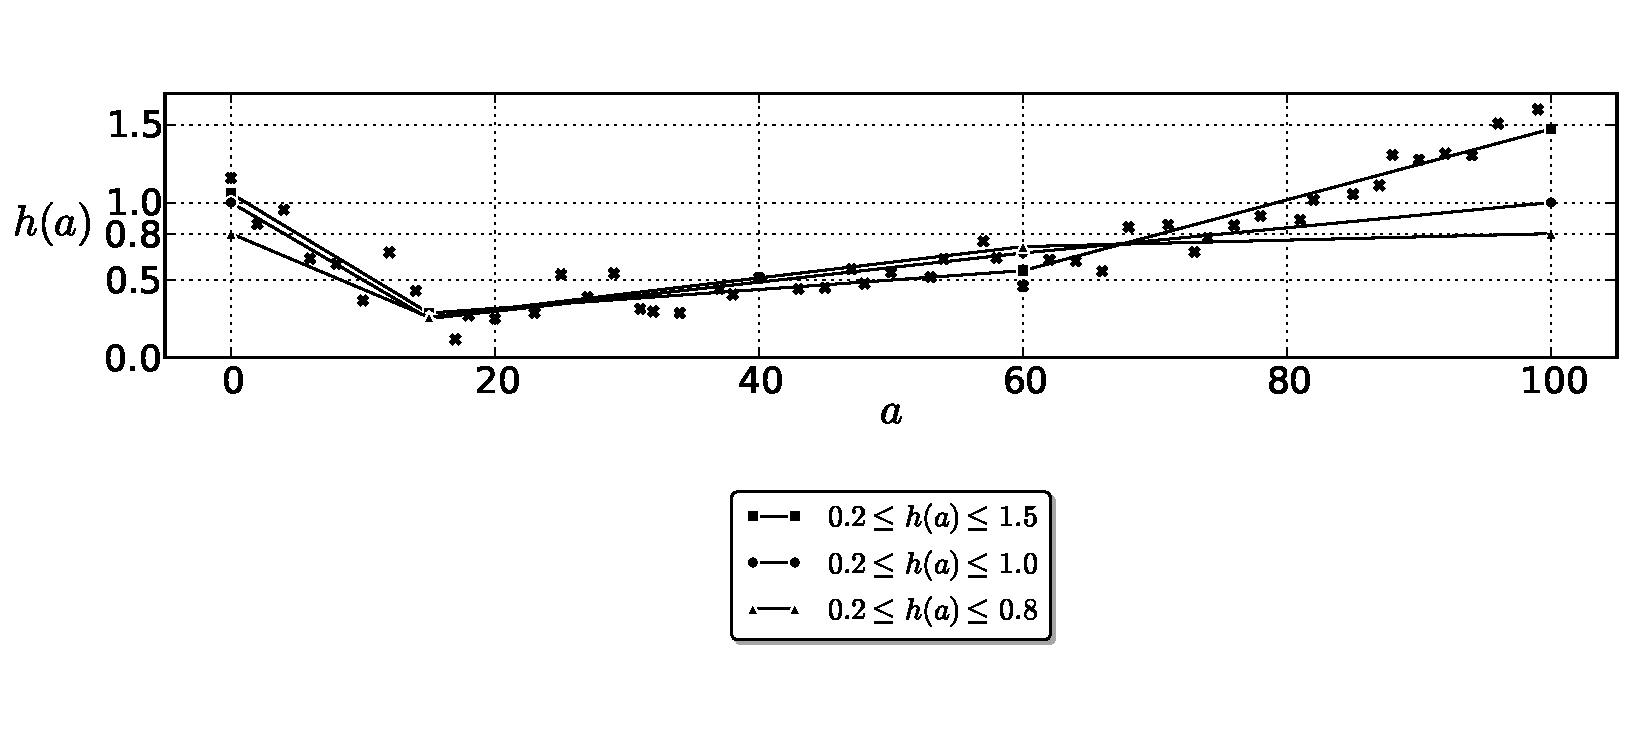
\includegraphics[width=\textwidth]{level_bound-smoothing-splines.pdf}
\caption[An informative prior on the upper and lower bounds of the
  age-specific hazard function $h(a)$.]{An informative prior on the
  upper and lower bounds of the age-specific hazard function $h(a)$
  changes the estimated hazard function dramatically for
  ages where the data are outside the bounds. For ages where the data
  are inside the bounds, the estimates are also affected, but to a lesser degree.}
\label{level-bounds-priors}
\end{center}
\end{figure}



Like the level value prior, this prior is also implemented as a
hard-soft constraint.  If the level bounds are $\ell_0 \leq h(a)
\leq \ell_1$, there is a hard constraint that replaces the spline with a
clipped version, $h^c(a) = \clip\left(h(a), \ell_0, \ell_1\right)$, and
also a soft constraint that ensures that the original spline is close to the clipped
spline in offset log-transformed space.

\section{Priors on monotonicity}

One common expert prior on age patterns is a strong belief that the
function is increasing or decreasing over a certain age
range. Mathematically speaking, these are priors on the sign of the
derivative of the age pattern.  For example, these priors can be implemented efficiently in
Bayesian Markov chain Monte Carlo (MCMC) computation by conditioning on the differences of the
age-specific hazard function $h(a)$:
\[
h(a) \geq h(a+1) \text{ for } a : a_s < a < a_e.
\]
The results of using such a prior are shown in
figure~\ref{monotone-age-pattern}.


\begin{figure}[h]
\begin{center}
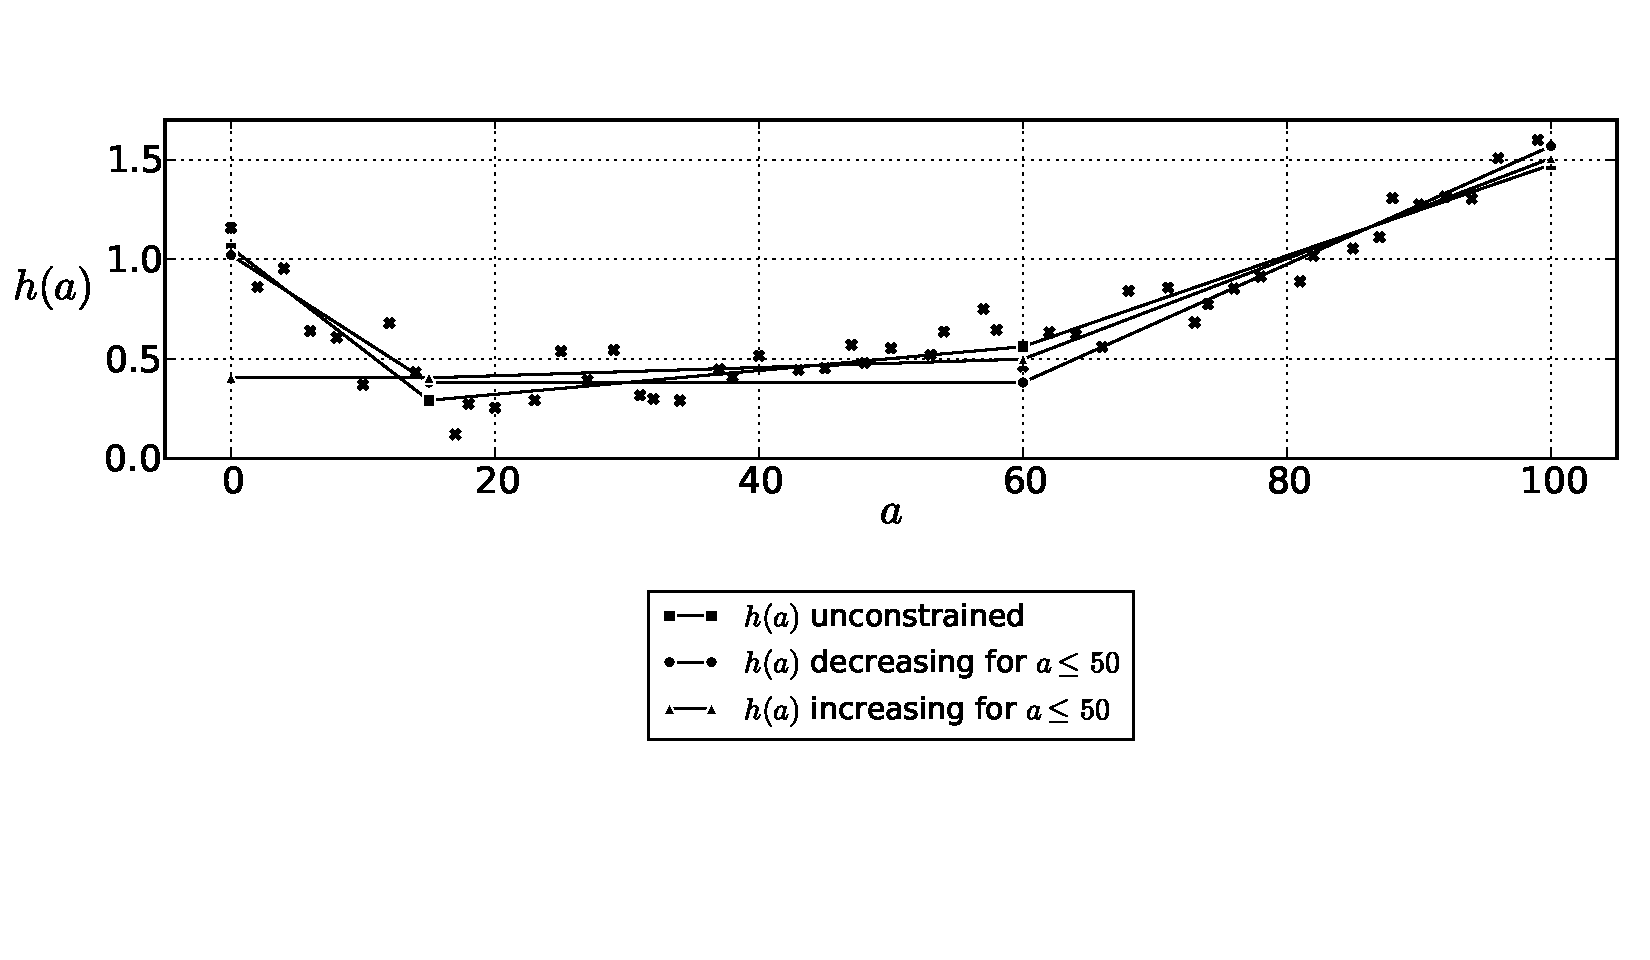
\includegraphics[width=\textwidth]{monotone-smoothing-splines.pdf}
\caption[An informative prior that the age pattern is increasing or
  decreasing across an age range.]{The expert belief that the age
  pattern is increasing or
  decreasing across an age range can also be implemented as a Bayesian
  prior.  When the prior is contrary to the data, the estimate will be
  as close to the data as possible while respecting the prior.  For
  example, the age-specific hazard function marked with triangles is the result
  of a prior belief that the age pattern increases from age $0$ to
  $50$ when confronted with data, shown as x-shaped marks that
  clearly decrease over this age range.}
\label{monotone-age-pattern}
\end{center}
\end{figure}


For computational efficiency, the increasing and decreasing
constraints are implemented as soft constraints.  For a constraint
that the function is decreasing between $a_s$ and $a_e$, I include the penalty
\[
\operatorname{clip}\left(\log h(a+1) - \log h(a), 0, 1\right) \sim \Normal(0, \epsilon^2)
\]
for a small value of $\epsilon$, like $\epsilon = 10^{-6}$.  This has
a fully Bayesian interpretation, encoding a belief that a decreasing age pattern is expected
and an increase of more than approximately $0.0003$\% is very surprising.


An area for future work comes from another common expert belief: that
the age pattern is unimodal.  This is conceptually clear, but
computationally it has proven more difficult to realize than
monotonicity.  While the monotonicity constraint maintains
log-concavity of the posterior distribution (if it was log-concave to
start with), a straightforward implementation of a unimodality
constraint will result in non-log-concave posterior distribution, even
if everything else is well behaved.  This suggests that the difficulty
in fitting such models is inherent in the local step method of the
MCMC algorithms I have been using.  Perhaps an alternative approach
such as the population Monte Carlo algorithm would be more successful.
Alternatively, there are some approximations of the unimodality
constraint that may be easier to optimize over.\cite{papp_shape_2012}

\section{Priors are not just for splines}
All three of the expert priors developed in this chapter are
applicable to any age-specific function derived from the compartmental
model in section~\ref{sys-dynamics}. Most importantly, the
age-specific prevalence $p(a) = C(a)/\left[S(a)+C(a)\right]$ can be augmented with expert
priors on level values (e.g., birth prevalence is $0$), level bounds
(e.g., no population has prevalence above $10$\%), and monotonicity
constraints (e.g., prevalence in increasing as a function of
age). Relative mortality risk $\frac{h_m(a)+h_f(a)}{h_m(a)}$ is another derived quantity
for which experts often have strong priors.

However, this sort of modeling requires care. The system dynamics
model enforces a precise consistency between the different
epidemiological rates, and making strong assumptions about one will
have implications for others.  Sometimes these implications are
counterintuitive.

As a practical matter, I recommend that modeling begin with as few
assumptions as possible to which expert priors may be added gradually. The
benefit of this is threefold.  First, fitting the model without all
the available expert knowledge allows the data to speak.  If the estimates
confirm the expert belief, that is reassuring, and if they show the
opposite, that is interesting. Second, the MCMC algorithm has a
pitfall: \emph{nonconvergence}. A quick way into this pit is
introducing inconsistent expert priors, for example, decreasing
prevalence and prevalence of $0$ at age $0$. By adding in expert
priors one at a time, the inconsistency that caused nonconvergence
will be more easily identified. Third, as with any model that produces
estimates from sparse and noisy data, it is essential to conduct a
sensitivity analysis to understand how influential modeling
assumptions are on the results.  The gradual addition of expert priors
will provide a starting point for this sensitivity analysis, showing
which expert priors are essential to obtaining reasonable results and
which are not as critical.

\section{Empirical priors on age patterns}
Another type of level prior worthy of separate exposition is that used
to implement the empirical Bayes approach that permits decomposing the
global estimation computation into region subcomputations that can be
run in parallel.  If estimates of the mean and standard deviation of
an age pattern are known for each age from a prior computation, this
information can be included in the age-specific hazard through a
penalty of the form
\[
h(a) \sim \Normal\left(\boldmu_{\text{prior}}(a),
\boldsigma_{\text{prior}}^2(a)\right).
\]

Since the model must cope with the order-of-magnitude differences of age-specific rates, it can be more robust to use an empirical prior relating the offset log-transformed rates:
\[
\log\left(h(a)+\epsilon\right) \sim \Normal\left(\log\left(\boldmu_{\text{prior}}(a)+\epsilon\right),
\left(\frac{\boldsigma_{\text{prior}}+\epsilon}{\boldmu_{\text{prior}}+\epsilon}\right)^2\right).
\]

\section{Statistical Models for Epidemiological Rates}
\label{theory-rate_model}

The key to connecting the systems dynamics model from
Chapter~\ref{theory-system_dynamics} to the evidence base collected
through systematic review is the \emph{rate model}.  This is a
statistical model, which has its core features defined by its
likelihood function.  By \emph{likelihood function}, I mean a
probability density function that assigns a value for the likelihood
of every possible (rate value, uncertainty)-pair for each setting of
the model parameter.  An examples will make this clearer, so I turn
now to the meta-analysis of population prevalence of schizophrenia in
adult males.  The forest plot in
Figure~\ref{fig:theory-rate_model-schiz_forest} shows the results of
combining $<<len(d['schiz_forest.json|dexy']['r'])>>$ studies using
$7$ different rate models.  As the figure demonstrates, the choice of
rate model can have a huge effect on the estimated uncertainty, and
can have a noticable effect on the estimated median as well. The
models I displayed produce point estimates ranging from
$<<d['schiz_forest.json|dexy']['min_est']>>$ to
$<<d['schiz_forest.json|dexy']['max_est']>>$, and uncertainty
intervals with widths ranging from
$<<d['schiz_forest.json|dexy']['min_spread']>>$ to
$<<d['schiz_forest.json|dexy']['max_spread']>>$.

In what follows, I will develop a collection of rate models, starting
with the simplest and then increasing complexity, while identifying
the benefits and drawbacks of each.  The models to come, in order, are
the binomial model, the beta-binomial model, the poisson model, the
negative binomial model, and three variants of the normal
model.

\begin{figure}
\begin{center}
\includegraphics[width=\textwidth]{theory-rate_model-schiz_forest_plot.png}
\end{center}
\caption{Forest plot summarizing $7$ alternative models for
  meta-analysis of adult male schizophrenia prevalence at
  population-level.  The median estimates range from
  $<<d['schiz_forest.json|dexy']['min_est']>>$ to
  $<<d['schiz_forest.json|dexy']['max_est']>>$, and the width of the
  $95\%$ HPD interval ranges from
  $<<d['schiz_forest.json|dexy']['min_spread']>>$ to
  $<<d['schiz_forest.json|dexy']['max_spread']>>$.}
\label{fig:theory-rate_model-schiz_forest}
\end{figure}

\subsection{Binomial Model}
My conceptually simplest model for rate data was built from the
binomial random variable, which follows the probability distribution
\[
\Pr[X=k\given n,\pi] = \binom{n}{k}\pi^n(1-\pi)^{n-k}
\]
I've used greek to emphasize that $\pi$ is the parameter, while $n$
and $k$ are data.

Although this equation may appear opaque, the intuition behind it is
simple: $n$ individuals were tested for a disease, and $k$ tested
positive. The formula then follows from the assumption that each
individual tested positive with probability $\pi$, and that 
knowing about the test results of any subset of individuals gives me
no information about what the test results the others were
(these events are ``independent'').

This distribution inspires a computationally tractable and
theoretically appealing rate model for a observed population rate of
$r$ from a population of size $n$:
\[
\dens(p,n\given \pi) \propto \pi^{\lfloor rn \rfloor}(1-\pi)^{\lceil (1-r)n \rceil}.
\]
Note that it is not necessary to include the term $\binom{n}{nr}$,
because this does not depend on the model parameter $\pi$. There is a
constant of proportionality, which is necessary to make this rate
model truely a probability density function for any $\pi$, but happily
I will never need to know this constant, and I have use the ``proportional to''
symbol $\propto$ instead of equality to emphsize this fact.

The funnel plot in Figure~\ref{fig:theory-rate_model-binom_funnel}
shows the predictive distribution of this rate model for $\pi=<<
d['binomial_model.json|dexy']['pi_binomial_funnel'] >>$.  It also shows
the potential problem with this approach: the data gathered by
systematic review are often much more dispersed than this
distribution predicts.

\begin{figure}[ht]
\begin{center}
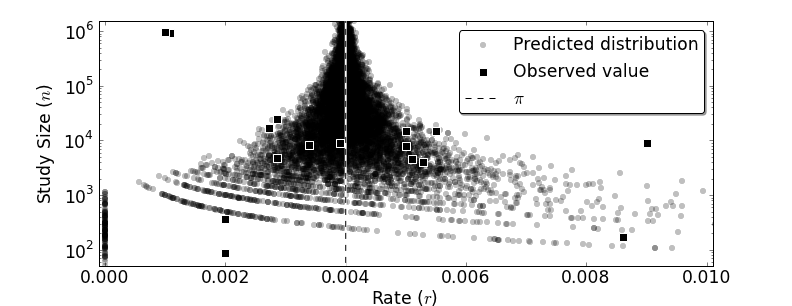
\includegraphics[width=\textwidth]{binomial-model-funnel.png}
\end{center}
\caption{Funnel plot showing predictive distribution for the binomial
  rate model with
  $\pi=<<d['binomial_model.json|dexy']['pi_binomial_funnel']>>$ (shown in
  blue), with data from systematic review for adult male schizophrenia
  prelvanece overlaid for comparison (shown in green).}
\label{fig:theory-rate_model-binom_funnel}
\end{figure}

All models are wrong, of course, so why does this model require
refinement? The answer is that is leads to unreasonably high
confidence when modeling noisy data.  If a study of
$<<d['binomial_model.json|dexy']['pop_A_N']>>$ people from in
subpopulation A finds prevalence of
$<<d['binomial_model.json|dexy']['pop_A_prev']*1000>>$ per thousand and
a study of $<<d['binomial_model.json|dexy']['pop_B_N']>>$ people in
subpopulation B finds $<<
d['binomial_model.json|dexy']['pop_B_prev']*1000 >>$, then the
binomial model predicts that a study of
$<<d['binomial_model.json|dexy']['pop_C_N']>>$ people in subpopulation
C will have prevalence of
$<<d['binomial_model.json|dexy']['pop_C_prev_per_1000']>>$, with
$95\%$ HPD interval
$<<d['binomial_model.json|dexy']['pop_C_ui_per_1000']>>$.  I have
no problem with the point estimate.  Picking the mean of the two
populations seems just right.  But the uncertainty interval lacks face
validity.  It would be much more reasonable to have an uncertainty
interval as large as $[1,7]$, instead of one as small as this.

One way to formalize this objection is through the posterior
predictive check, an in-sample goodness-of-fit test that can be done
graphically.  Figure~\ref{fig:theory-rate_model-binom_ppc} shows the
posterior predictions of the binomial model when it is fit to the
adult male schizophrenia dataset, together with the data itself.  The
model predictions are clearly compressed, and trusting the results of
such a model will lead to inappropriate certainty in the face of noisy
data.

\begin{figure}[ht]
\begin{center}
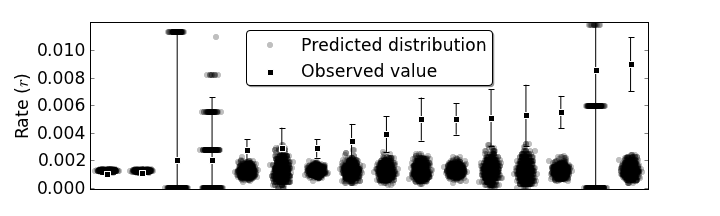
\includegraphics[width=\textwidth]{binomial-model-ppc.png}
\end{center}
\caption{Posterior predictive check for binomial model fit to adult
  male schizophrenia data.  Blue shows 1000 draws from the posterior
  distribution of the binomial model, and green shows the input data.}
\label{fig:theory-rate_model-binom_ppc}
\end{figure}




\subsection{Beta-binomial model}
A theoretically appealing extension to the binomial model (which also
does not work for my purposes) is the beta-binomial model.  I will
develop it in this section, to motivate the following sections.

Formally, the beta binomial random variable is given by the following
probability distribution
\begin{align*}
\Pr[X = k\given n, \alpha, \beta] 
  &= \int_{\pi}\dens(\pi\given \alpha, \beta) \binom{n}{k}\pi^k(1-\pi)^{n-k}
d\pi\\
\dens(\pi\given \alpha, \beta) &\propto \pi^{\alpha-1}(1-\pi)^{\beta-1}
\end{align*}

The intuition behind this model is simpler than the equation, however.
As in the binomial model, each individual tests positive for the condition independently
with a probability $\pi$, but now $\pi$ itself is a random variable,
distributed according to a beta distribution with parameters $\alpha$
and $\beta$. The beta distribution is given by 
\[
\dens(\pi\given \alpha, \beta) =
\frac{\Gamma(\alpha+\beta)}{\Gamma(\alpha)\Gamma(\beta)}\pi^{\alpha-1}(1-\pi)^{\beta-1}
\]
and has a high degree of flexibility.  It also always takes values
between zero and one, making it an appropriate distribution for a
probability.  Figure~\ref{fig:theory-rate_model-beta} shows the
probability density of the beta distribution for several combinations
of $\alpha$ and $\beta$.
\begin{figure}[ht]
\begin{center}
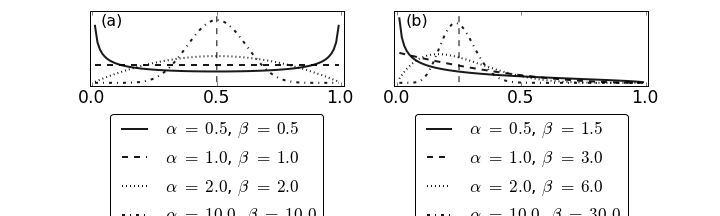
\includegraphics[width=\textwidth]{beta-distribution.png}
\end{center}
\caption{Probability density for the beta distribution for a range of
  $\alpha$ and $\beta$ values. Dashed black line shows expected value,
which is $.5$ for all distribution in a) and $.25$ for all in b).}
\label{fig:theory-rate_model-beta}
\end{figure}

The beta binomial distribution inspired the following rate model for
an observed population rate of $r$ from a population of size $n$:
\[
\dens(r,n\given \alpha, \beta) \propto \int_{\pi}
\pi^{\alpha-1}(1-\pi)^{\beta-1} \pi^{\lfloor rn\rfloor} (1-\pi)^{\lceil (1-r)n\rceil}
d\pi.
\]

This model extends the binomial model in a way analogous to how a
random effects model in linear regression.  By introducing an
additional dimension in to the parameter space, it is able to capture
the dispersion beyond the binomial model that I have observed
empirically in funnel plots of real data
(Figure~\ref{fig:theory-rate_beta-binomial-funnel} shows the beta
binomial funnel plot, as well as the posterior predictive check for
this model on the same data as used in
Figure~\ref{fig:theory-rate_model-binom_ppc}.

\begin{figure}[ht]
\begin{center}
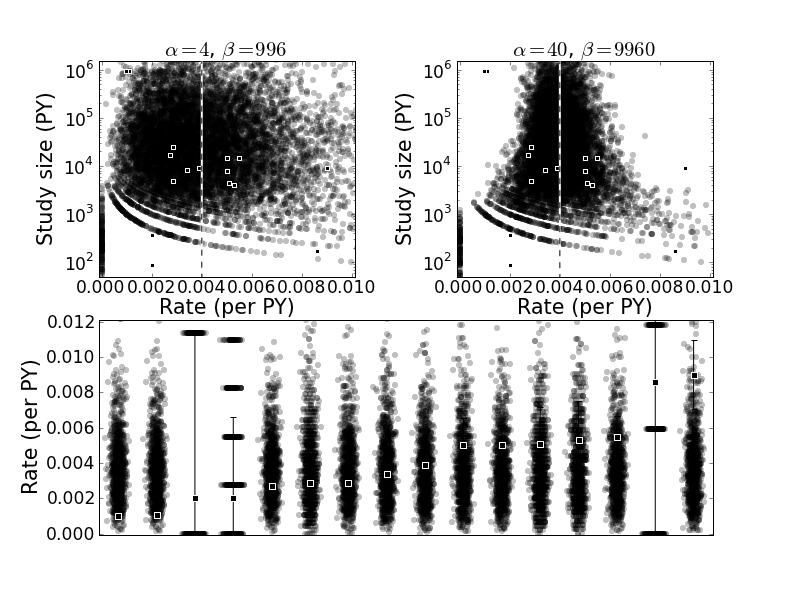
\includegraphics[width=\textwidth]{beta-binomial-funnel.png}
\end{center}
\caption{Funnel plot and posterior predictive check for beta binomial model.}
\label{fig:theory-rate_beta-binomial-funnel}
\end{figure}

This model addresses the theoretical shortcoming raised in the
previous section: if studies of
$<<d['beta_binomial_model.json|dexy']['pop_A_N']>>$ people show prevalences
of $<<d['beta_binomial_model.json|dexy']['pop_A_prev']*1000>>$ and
$<<d['beta_binomial_model.json|dexy']['pop_B_prev']*1000>>$ per thousand,
then the posterior distribution of the beta binomial model has mean
$<<d['beta_binomial_model.json|dexy']['pop_C_prev_per_1000']>>$ with 95\%
HPD interval $<<d['beta_binomial_model.json|dexy']['pop_C_ui_per_1000']>>$,
which seems quite reasonable.

The great shortcoming of the beta binomial model is computational.  As
will be elaborated in Chapter~\ref{theory-numerical_algorithms}, there
is no closed-form solution to the integral in the probability density
for the beta binomial model.  Evaluating it requires introducing a
latent variable for each of the data points in the likelihood.  This
simply had too much cost for the numerical algorithms and
computational infrastructure available.  So my search
continued.

\subsection{Other count models}
There are two traditional approximations to the binomial distribution,
depending on how large $k$ is in relation to $n$.  When $k/n$ is
large, the normal distribution is used, and when $k/n$ is small, the
binomial is similar to the Poisson distribution.

Since I expect to usually be in a ``small $k/n$'' setting, I will not
develop the normal model in detail now, although in the next section I
will develop to model based on monotonic transformations of the normal
distribution which include a normal model as a special case.

The Poisson distribution is given by the the equation
\[
\Pr[X=k] = \frac{\lambda^k e^{-\lambda}}{k!},
\]
and it can be understood intuitively as the number of times a
``memoryless'' event occurs in a unit time period.  Setting $\lambda =
\pi n$ produces an approximation to the binomial distribution, which
is quite accurate for large $n$ and small $k$.
Figure~\ref{fig:theory-rate_model-poisson_approx_to_binom}
demonstrates how precise this approximation can be when approximating
a binomial distribution with
$n=<<d['poisson_model.json|dexy']['n_small']>>$ and
$\pi=<<d['poisson_model.json|dexy']['pi_true']>>$.

\begin{figure}
\begin{center}
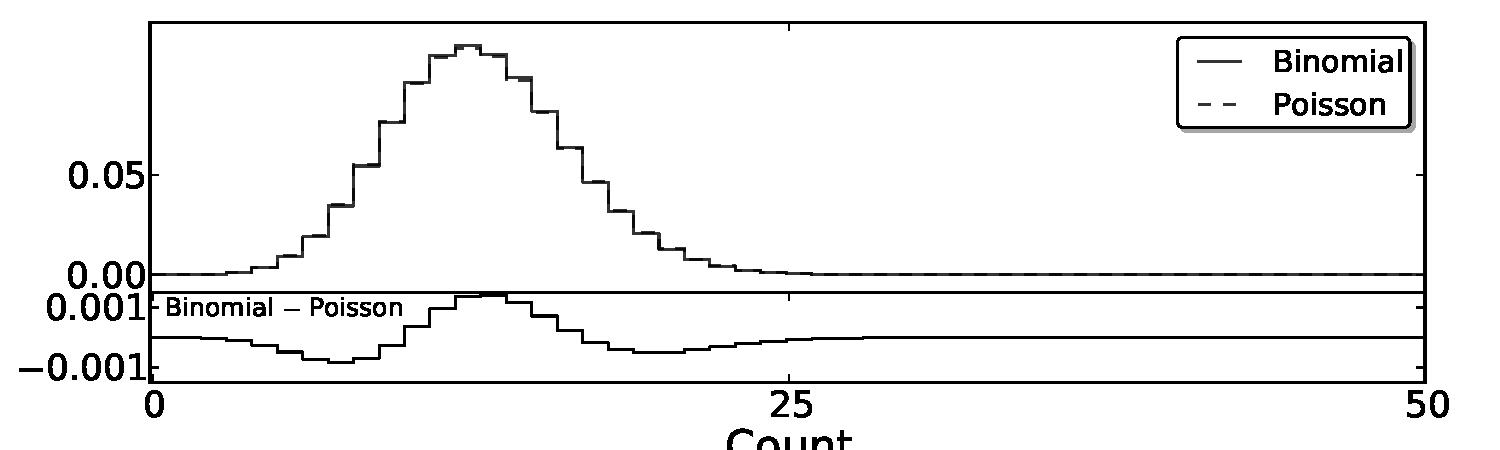
\includegraphics[width=\textwidth]{poisson_approx_to_binom.png}
\end{center}
\caption{The Poisson distribution approximates the binomial
  distribution very closely. Here a binomial distribution with
  $n=<<d['poisson_model.json|dexy']['n_small']>>$ and
  $\pi=<<d['poisson_model.json|dexy']['pi_true']>>$ is approximated by
  a Poisson distribution with parameter
  $\lambda=<<d['poisson_model.json|dexy']['n_small'] *
  d['poisson_model.json|dexy']['pi_true']>>$.  The difference between
  the distributions is shown in the lower panel, since the curves in
  the upper panel are almost indistinguishable by eye.}
\label{fig:theory-rate_model-poisson_approx_to_binom}
\end{figure}

Because of the similarity of these distributions, the Poisson model,
is defined by
\[
\dens(r,n\given \pi) \propto (\pi n)^{\lfloor rn\rfloor} e^{-\pi n}.
\]
It is subject to all of the concerns raised about the
binomial model regarding inappropriately low levels of uncertainty
when modeling rates with non-sampling variation at the level typically
gathered in systematic review.

There is one key benefit to this model, compared to the binomial and
beta-binomial models, however.  The Poisson model assigns a
theoretically justified and non-zero likelihood to rates of more than
one.  Although prevalence is always less than one, it is theoretically
possible to have incidence rates more than one, and remission rates
are often more than one (per person-year).

Another benefit from this approach is to be found in its
over-dispersed variant.  This distribution
is called the negative binomial distribution (named after the formula
that the proves it does indeed sum to one).  Unlike the beta-binomial
distribution, it \emph{does} have a closed form (if you consider the gamma function ``closed''):
\[
\Pr[X = k\given \pi, \delta] = \frac{\Gamma(k+\delta)}{\Gamma(\delta)k!}
\left(\frac{\delta}{\pi+\delta}\right)^\delta \left(\frac{\pi}{\pi+\delta}\right)^k
\]

However, this closed form obscures the intuition behind the negative
binomial distribution, which is quite similar to the intuition behind
the beta-binomial distribution, although less clear from the
name. Through a bit of algebra, the negative binomial distribution can
be represented as a hierarchical model, where the observed data comes
from a Poisson distribution, and the parameter of the Poisson
distribution is itself a random variable that comes from a gamma
distribution:
\begin{align*}
X\given \pi &\sim \Poisson(\pi)\\
\pi &\sim \GammaDist(\mu, \delta)
\end{align*}
Here the Gamma distribution is defined by (TK reparameterize to match above)
\[
\dens(x; k,\theta) =
x^{k-1} \frac{e^{-x/\theta}}{\theta^k \, \Gamma(k)}.
\]
Through this lens, the negative binomial model can be interpreted as a
nature adaptation of the traditional random effects model in linear
regression to the Poisson case, where each observation comes from a
different Poisson model and the Poisson parameter of these models are
all drawn from a common Gamma distribution.

Thus a rate model based on it provides benefits in handling
non-sampling variation similar to those demonstrated for the beta
binomial distribution above, but in a formulation that is much less
demanding computationally.  The negative-binomial rate model for
observing a rate of $r$ in a population of size $n$ is:
\[
\dens(r,n\given \pi, \rho) \propto \frac{\Gamma(\lfloor rn\rfloor+\rho)}{\Gamma(\rho)} (1-\pi)^\rho \pi^{rn}.
\]

A difficultly I have observed in practice with the negative binomial
model is in the realm of numerical algorithms.  My experience has been that these
likelihoods lead to models that are simply harder to fit than
traditional normal models.  Nonetheless, the negative binomial model
has been the primary tool in the likelihod modeling for the
applications to be presented in Chapters~\ref{practice-all-examples}.

Chapter~\ref{TK} will examine the properties of numerical algorithms
for fitting the negative binomial model in more detail, but one
approach which has helped substantially is imposing an informative
prior on the over-dispersion parameter of the negative binomial
distribution.  Because it seems unreasonable to impose a very
informative prior on the over-dispersion parameter, I have limited the
possibilities to augmenting the hierarchical formulation of the
negative binomial model above with the following:
\[
\log_{10} (\delta-5) \sim \Normal\left(\mu_{\log\delta}, .25^2\right),
\]
with $\mu_{\log\delta} = 1, 2, 3$.  The results of adding this
prior are contrasted with the results vanilla negative binomial model
(with an uninformative prior on $\delta$) in
Figure~\ref{fig:theory-rate_model-neg_binom_priors}, which shows that
a belief a priori that the observations is more over-dispersed leads
to a posterior estimate where the predicted rate have more
uncertainty, as expected.

\begin{figure}
\begin{center}
\includegraphics[width=\textwidth]{neg_binom_priors.png}
\end{center}
\caption{Forest plot of a simulation experiment demonstrating the
  effect of a weakly informative prior on the negative binomial model
  posterior.  Sixteen data points simulated from a negative binomial
  distribution are fit with negative binomial models, with $5$
  different priors on the dispersion term $\delta$.  The informative
  prior of $\delta = \infty$ reduces the negative binomial model to
  the poisson model, and for this case the uncertainty interval does
  not contain the truth.  All of the weakly informative priors do
  contain the truth, however.  Replicating this simulation
  $<<d['neg_binom_sim.json|dexy']['replicates']>>$ times yielded mean
  bias of
  $\E[\pi_{\true}-\pi_{\median}]=<<d['neg_binom_sim.json|dexy']['bias']['pi']>>$
  and root mean squared error of
  $\RMSE[\pi_{\true}-\pi_{\median}]=<<d['neg_binom_sim.json|dexy']['rmse']['pi']>>$;
  the uncertainty interval contained the $\pi_{\true}$ value with probability
  $<<d['neg_binom_sim.json|dexy']['percent_coverage']['pi']>>$.}
\label{fig:theory-rate_model-neg_binom_priors}
\end{figure}

\subsection{Transformed normal models}
Some epidemiological data is not count data at all.  Duration studies
and studies measuring the relative risk of mortality are two that come
up frequently in systematic review.  For duation data, a normal model
has been quite sufficient, and a log-normal model has proven
appropriate for modeling relative risk data, which can be thought of
as a ratio of count variables.

Transformed normal models have also been used for mortality rates in
the past [ref including GK TK], and are worthy of continued consideration for
modeling the incidence, prevalence, remission, and mortality as an
alternative to the negative binomial.

In this section, I will develop a general transformed normal model,
and compare it to the negative binomial model.  The adjective
``transformed'' refers to a function which I will keep quite general
for now, requiring it only to be increasing and differentiable,
i.e. for any $x > y$ the transformation $f$ must have $f(x) > f(y)$
and $f'(x)$ must be defined.  Then transformed normal model will be
derived from the normal distribution, defined by the probability
density
\[
\dens(x\given \pi, \sigma) \propto \frac{1}{\sigma} \exp\left\{ -\frac{(x-\pi)^2}{2\sigma^2} \right\}.
\]

For any increasing, differentiable function $f$, this distribution can be converted to
an $f$-transformed normal model with probability density
\[
\dens(r,s\given \pi, \sigma, f) \propto \exp\left\{-\frac{\left(f(r)-f(\pi)\right)^2}{2\left((sf'(r))^2+\sigma^2\right)}\right\},
\]
where $s$ is the standard error of the rate $r$, which is more
convenient that the effective sample size $n$ in this case. The
denominator of the exponent deserves some additional discussion.  For
the identity function $f(x) = x$, the derivative $f'(x) = 1$, and the
denominator simplifies to $2(s^2 + \sigma^2)$, a familiar ``inverse
variance'' weighting where $\sigma$ is a random effect to account for
over-dispersion.  When $f$ is a more complicated function, the term
$sf'(r)$ approximates the standard error of the transformed value
$f(r)$.  Although more sophisticated approximations are possible,
experience dictates that the non-sampling variation (parameterized by
$\sigma$) is always larger than the chance variation, so a simple
approximation of the chance variation is sufficient.

Some common transformations $f$ used in related work yield the
lognormal model ($f(x) = \log x$) the logit model ($f(x) = \logit x$)
and the probit model ($f(x) = \probit x$).  All of these approaches
have a significant drawback, however.  The transform is not defined
for $x=0$, so these models cannot use data showing rates of zero.
There are two common methods to fix this, dropping all zeros, and
adding a small offset.  Dropping measurements of zero is clearly
problematic, as it leads to systematic bias in the data that remains
and produces estimates larger than they should be.  This is especially
true for high quality studies which focus on the age pattern of a
disease, where it is quite reasonable for some age groups to have zero
cases observed.  The effect of dropping zeros is to overestimate the
rates in these age groups.

Adding a small amount, such as $0.5$ is an alternative solution, and
indeed, this is the approach taken for cause-specific mortality estimation
in GK [ref TK].  The selection of the offset can appear ad hoc,
however.

Within the framework of the transformed normal model, there is
room to put the solution on firm theoretical foundations.  For
example, by taking $f_\zeta(x) = \log(x + \zeta)$, I obtained the
``offset log transformed model'', which does allow rates of zero,
simply by taking a positive value for $\zeta$.  This model will not be
used extensively in the example application to come later in this
book, but it seems like a promising approach.  It is particularly
appealing in the way it decomposes the non-sampling variation into an
additive error $\zeta$ and a multiplicative error $\sigma$, and I
expect that it will prove useful in the future.  For completeness,
here is the probability density for the offset log transformed model:
\[
\dens(r,s\given \pi, \sigma, \zeta) \propto
\exp\left\{-\frac{\left(\log(r+\zeta)-\log(\pi+\zeta)\right)^2}{2\left(\left(\frac{s}{r+\zeta}\right)^2+\sigma^2\right)}\right\}.
\]

\subsection{Lower-bound data model}
Cause-specific mortality rates are a special case among the
epidemiological rates available for integrative systems modeling of
disease in a population.  These data come from carefully processing of
vital registration system output, from verbal autopsy stdies, and from
some other sources. But unlike incidence, prevalence, and remission
data, there is no rate or ratio in the compartmental model that
corresponds directly to this quanbtity.  This is because of the ``one
death has one cause'' mantra of biomedical theory.  The excess
mortality rate in the system dynamics model from Chapter TK is not
entirely compatible with this idea.

Cause-specific mortality data nonetheless provides \emph{some}
information, and should be used in an integative model if it is
available, especially if other sources are sparse and noisy (they
always are, in my experience).  By decomposing the excess mortality
into part that is ``cause-of-death mortality'' and residual excess
mortality, i.e. $f = f_{cod} + f_{non}$, it follows that $CSMR =p
\cdot f_{cod} \leq p\cdot f$, so the following lower bound model is
appropriate:
\[
\dens(CSMR \given \pi,\delta)
=
\begin{cases}
\calD(CSMR, \pi, \delta), &\qquad\text{if } \pi-CSMR \geq 0;\\
\calD(\pi, \pi, \delta), &\qquad\text{otherwise.}
\end{cases}
\]

\subsection{Summary and Comparison}
This section has developed $7$ alternative rate models, all with
benefits and drawbacks.  The binomial model is simple and
theoretically appealing, but does not handle non-sampling variation,
producing over-confident estimates in the face of noisy data.  The
beta binomial model deals with over-dispersion through a theoretically
appealing extension to the binomial model, but it is too
computationally demanding to use in my applications.  The poisson
model is a close approximation to the binomial model, and has all of
the drawbacks except it can handle rates greater than 1, which is
important for modeling remission rates.  So it is the negative
binomial model, which extends the poisson model analogously to the way
the beta binomial model extends the binomial model that I have settled
on for most of the applications to follow, using it to model
incidence, prevalence, remission, excess-mortality, and cause-specific
mortality. It is not as ammenable to analysis as I would like however,
and sometimes benefits from weakly informative priors on the
over-dispersion parameter, an undesirable feature that slows down
analysis by requiring sensitivity analysis.  Transformed normal models
are a promising alternative approach, and I have used the normal model
for duration data in some of the following examples, as well as
the lognormal model for standardized mortality rate data and relative
mortality risk data. The offset log transformed model seems
particularly promising as an alternative to the negative binomial
model, and understanding its statistical and computational
characteristics is a promising direction for future research.

TK some sort of comparison: simulation study? posterior predictive
checks? something analogous to SMART counties in small areas
estimation?

\chapter{Statistical models for heterogeneous age groups}
\chapterprecis{Abraham D. Flaxman}
With a full development of statistical rate models for a single age
group behind us, and the mathematical model for an age-specific rate
function laid out as well, this section turns to a peculiar feature of
population rate metaregression: the wide variety of age groups reported
in the literature.

A typical example of the heterogeneity in age groups is shown in for
the systematic review results on atrial fibrilation (AF)
prevalence\cite{TK_AF_report_reference} in
Figure~\ref{age-group-model-af-age-groups}.  The midpoint of the age
group is scattered against the width of the age group.  Simply put,
there is no standard set of age groups for AF research, and different
studies report results with different age groups. Unfortunately, this
phenomenon is far from unique to AF.

\begin{figure}[h]
\begin{center}
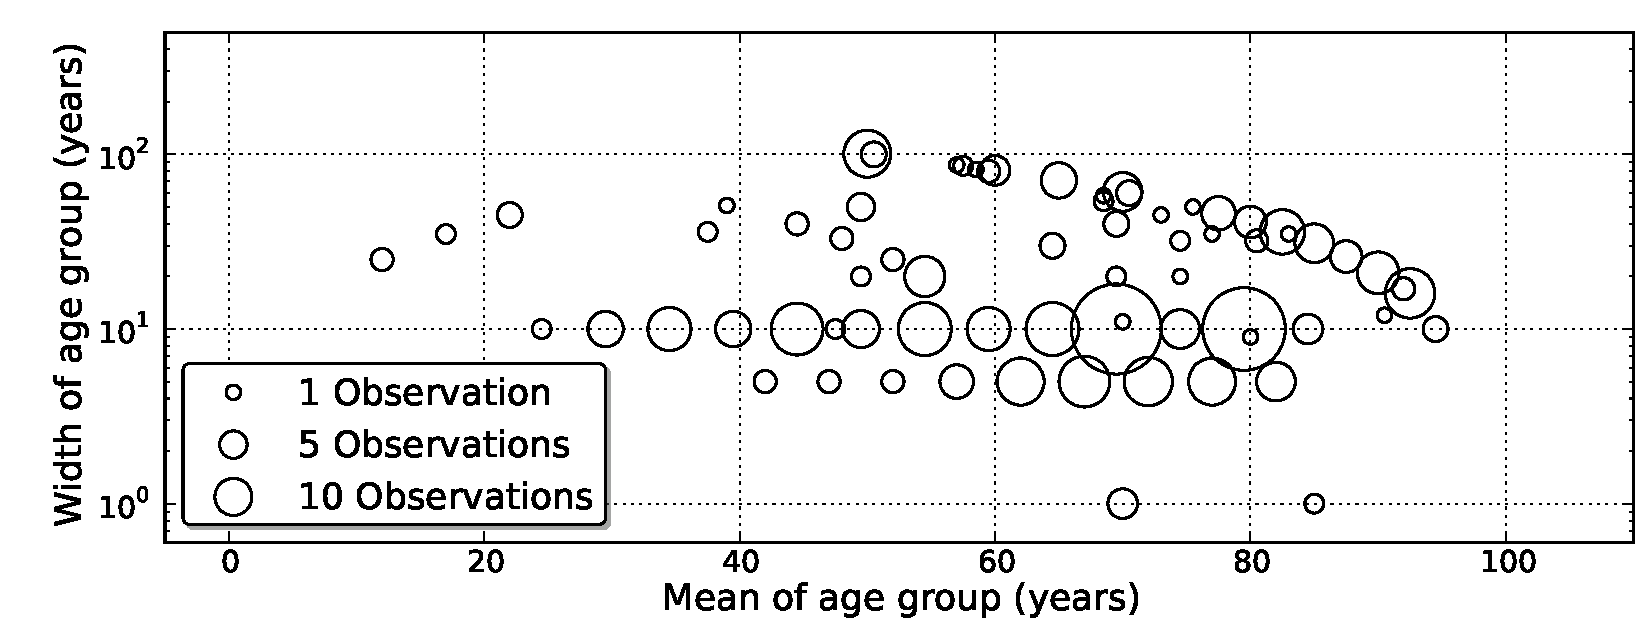
\includegraphics[width=\textwidth]{af_age_groups_scatter.pdf}
%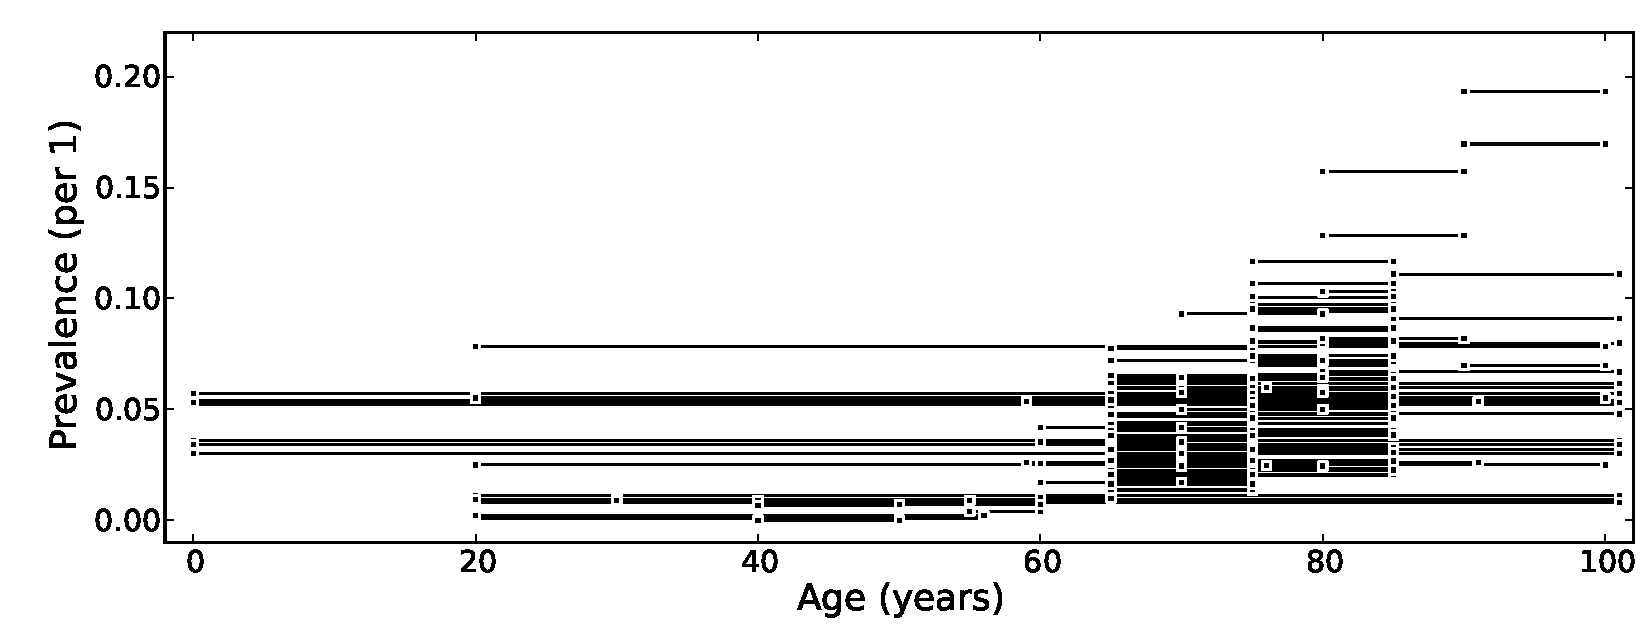
\includegraphics[width=\textwidth]{af_ages_intervals.pdf}
\end{center}
\caption{Mean and spread of age groups in the prevalence data
  collected from a systematic review of atrial fibrilation. The
  size of the circle shows how many observations of this age group
  were found in systematic review. There were
  $586$ rows of prevalence data
  extracted, but the most common age group accounted for only
  $68$ rows.}
\label{age-group-model-af-age-groups}
\end{figure}

This variation in reporting would not be problematic if I had access
to the microdata from all of the systematic review studies.  For
example, using microdata from a national health information system or
from a demographic household survey, I could simply tally the
prevalence rates by single-year age groups.  Although each individual
rate gathered in this way would have high variability, the rate model
from Chapter~\ref{theory-rate_model} combined with the spline model
for an age-specific hazard function from Chapter~\ref{theory-age_pattern_model} would
work together to produce an estimate that is as uncertain as it should be.

Re-analysis from microdata is occasionally implemented in a GBD study,
however it is often not an option.  I expect the use of microdata
re-analysis to become more frequent in national and subnational
settings.  In the more common situation where rate microdata are not
available, the rates cannot be retallied into homogeneous age groups,
and an alternative approach is needed.

There are several statistical approaches which I have considered, and
they will be compared and contrasted in this section.  Before getting
into the details, however, it is worthwhile to examine theoretically
the way that age grouping functions.

I begin with a simple mechanistic model of the age grouping process.
A study conducts some sort of measurement on a population of
individuals who are all of different ages and then the
epidemiological rate or rates of interest are tallied for age groups
selected in some context dependent manner. If the study was a
prevalence study using a full census sample, for example, and if I use
$r_{a_0,a_1}$ to denote the rate for age group $(a_0, a_1)$ and
$n_{a_0,a_1}$ to denote the subpopulation size of age group
$(a_0,a_1)$, then the identity
\[
n_{a_0, a_2} = n_{a_0,a_1} + n_{a_1,a_2}
\]
says nothing more complicated than that the size of the subpopulation
of age at least $a_0$ and less than $a_2$ is the sum of the size of
the subpopulation between age $a_0$ and $a_1$ and the size of the
subpopulation between age $a_1$ and $a_2$.  Applying the same
observation to the part of these subpopulations that have the condition
of interest yields the following identity:
\[
r_{a_0,a_2} = r_{a_0,a_1}\frac{n_{a_0,a_1}}{n_{a_0,a_2}} + r_{a_1,a_2}\frac{n_{a_1,a_2}}{n_{a_0,a_2}}. 
\] 
In a limiting case of a very large population with very fine age
intervals, this becomes:
\[
r_{a_0,a_2} = \int_{a=a_0}^{a_2} r_{a,a+\d a}\frac{n_{a,a+\d a}}{n_{a_0,a_2}}\d a.
\]
Undoubtedly all real studies are more complicated than this full
census of prevalence, but this is a starting point for conceptualizing
where age-grouped rates come from.  Roughly, they are integrals over
instantaneous rates for infinitesimal age groups.

\section{Overlapping age group data}
\label{theory-age_group_model-overlapping_data}
This section explores an examples of overlapping age group data
collected in systematic review through graphical statistics.  The
primary way I like to display overlapping age group data is shown in
Figure~\ref{theory-age_group_model-dismod_data_plot} as horizontal
lines on a plot of age versus rate value.  The level of the bars shows
the rate value, while the width of the bars shows the range of ages
included in the age group. It is often informative to augment these
lines with error bars, showing the uncertainty reported for each rate
value, but for this section I have left out the representation of
uncertainty to keep the plots as simple as possible.

\begin{figure}[ht]
\begin{center}
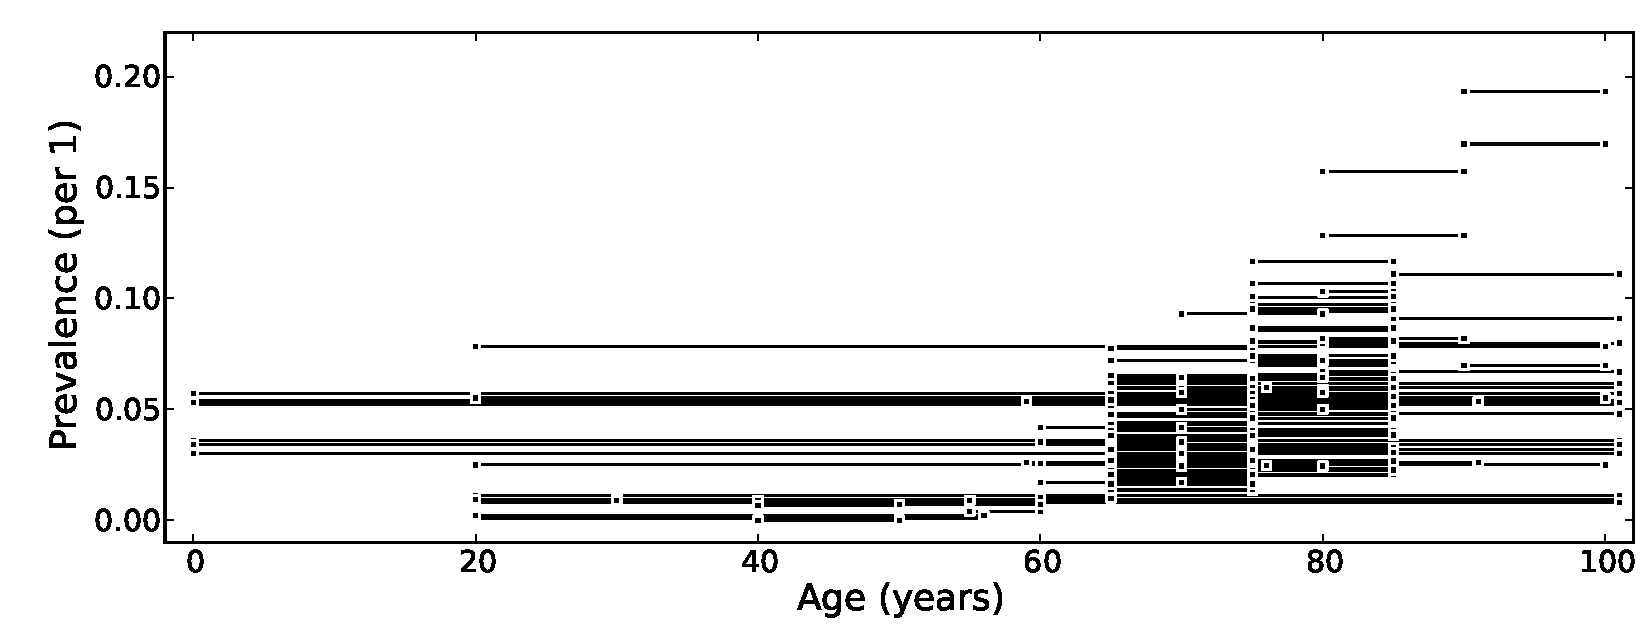
\includegraphics[width=\textwidth]{af_ages_intervals.pdf}
\caption{The systematic review of the descriptive epidemiology of
  atrial fibrilation included $155$ observations of disease prevalence for the United States.
 The prevalence level and age group of
  each observation is shown above as a horizontal bar, with the
  position of the bar along the $y$-axis representing the prevalence
  level and the endpoints along the $x$-axis representing the start and
  end of the age group.  The data shows heterogeneity by age that is
  typical for these systematic review results, which clearly increases with
 with age.  }
\label{theory-age_group_model-dismod_data_plot}
\end{center}
\end{figure}

Each of the horizontal lines in
Figure~\ref{theory-age_group_model-dismod_data_plot} can be
represented as a triple $({a_s}, {a_e}, r)$, where $a_s$ is the
starting age of the age group, $a_e$ is the ending age of the age
group, and $r$ is the rate observed for this age group.

A brief word about ${a_e}$ is in order here.  Often in the
epidemiological literature, the ending ages are described in a
unit-dependent fashion, for example age group 10-14.  This is intended
to mean from the first day of age 10 to the last day of age 14.
However, this notation can be a hindrance when dealing with age
resolution finer than one year, a situation that comes up when studying
neonatal conditions.  For this reason, I prefer the approach that
takes the end age of the interval to be the first age where an
individual is no longer part of the group.  In the case above, I would
say ${a_e} = 15$.


With a firm understanding of the sort of overlapping age group data
that arises in systematic review, I now turn to developing and
analyzing a series of models for the meta-analysis of the data.  There
are five that I will consider: the midpoint model, the disaggregation
model, the midpoint-with-covariate model, the age-standardizing model,
and the age-integrating model.  The age-standardizing model is the
balance of theoretical foundations, practical implementability, and
empirical success that is used in the second half of this
book.

\section{Midpoint model}

The simplest approach to modeling data with heterogeneous age
intervals, is to apply each rate measurement to the midpoint of the
age group it measured.  This is trivial operationally, but it is also
theoretically justified through a ``trapazoidal rule'' integration.

In practice, this approach is quite accurate for modeling a
disease rate that changes slowly as a function of age.  However, it
becomes inaccurate when modeling rates that change more
rapidly.  The typical setting in applications in the second half of
this book will include a few studies that focus on age patterns and
hence have narrow age groups, together with many other studies
that focus on other aspects of disease epidemiology.  Thus the
relevant setting to consider how these models are inaccurate is where
there are a few small age group studies and many large age group
studies.

Mathematically, the formulation is as follows: let $h(a)$ be a
process-model for the age-specific function (e.g a spline model
from Chapter~\ref{theory-age_pattern_model}, or the age-specific prevalence function derived from the solution to the system of differential equations from Chapter~\ref{sys-dynamics}), and let $\dens(r,n\given
\mu,\rho)$ be a data-model for the observed level (e.g the probability
density function for negative-binomial rate model from
Chapter~\ref{theory-rate_model}).
Then the likelihood of an observation of rate $r_i$ with effective
sample size $n_i$ for age group $({a_s}_i, {a_e}_i)$ is simply
$\dens\left(r_i, n_i \given h\left(\frac{{a_s}_i+{a_e}_i}{2}\right),
\rho\right)$. Equivalently, in ``blackboard notation,'' using
$\scD(\mu, \rho; n_i)$ to denote the rate model distribution, I can
write
\begin{align*}
r_i &\sim \scD\left(h(a_i), \rho; n_i\right),\\
a_i &= \frac{{a_s}_i+{a_e}_i}{2}.
\end{align*}
This formulation will be convenient for comparison with the other models of age groups to come.

To understand how accurately age group models like the midpoint model
can estimate, I used simulation.  The precise details are defered
until Section~\ref{agm-compare}, but, since this simulation is also used for the
figures that follow, I will describe it in brief here.  First, I
selected an age-specific hazard function as ground truth.  Then I
generated noisy measurements, from a mixture of regularly spaced
$10$-year age groups and uniformly random age groups.  For each
measurement, I chose a random population structure, and integrated the
true age-specific hazard to find the true rate for the age group.
Then I sampled from a negative binomial distribution with this true
rate as the mean, and a fixed overdispersion parameter to obtain noisy
data, which I used in the age group model.  Since ground truth is
known in this simulation, I can compare the model estimates to the
truth graphically as well as quantitatively.

Figure~\ref{midpoint} compares the estimate produced by the midpoint
model to ground truth through simulation using two different
age-specific hazard functions as ground truth.  When the age-specific
hazard varies little as a function of age, as shown in panel (a), the
estimated hazard function is quite accurate.  But when the age-specific hazard function
varies substantially, as shown in panel (b), the estimate is biased.


\begin{figure}[h]
\begin{center}
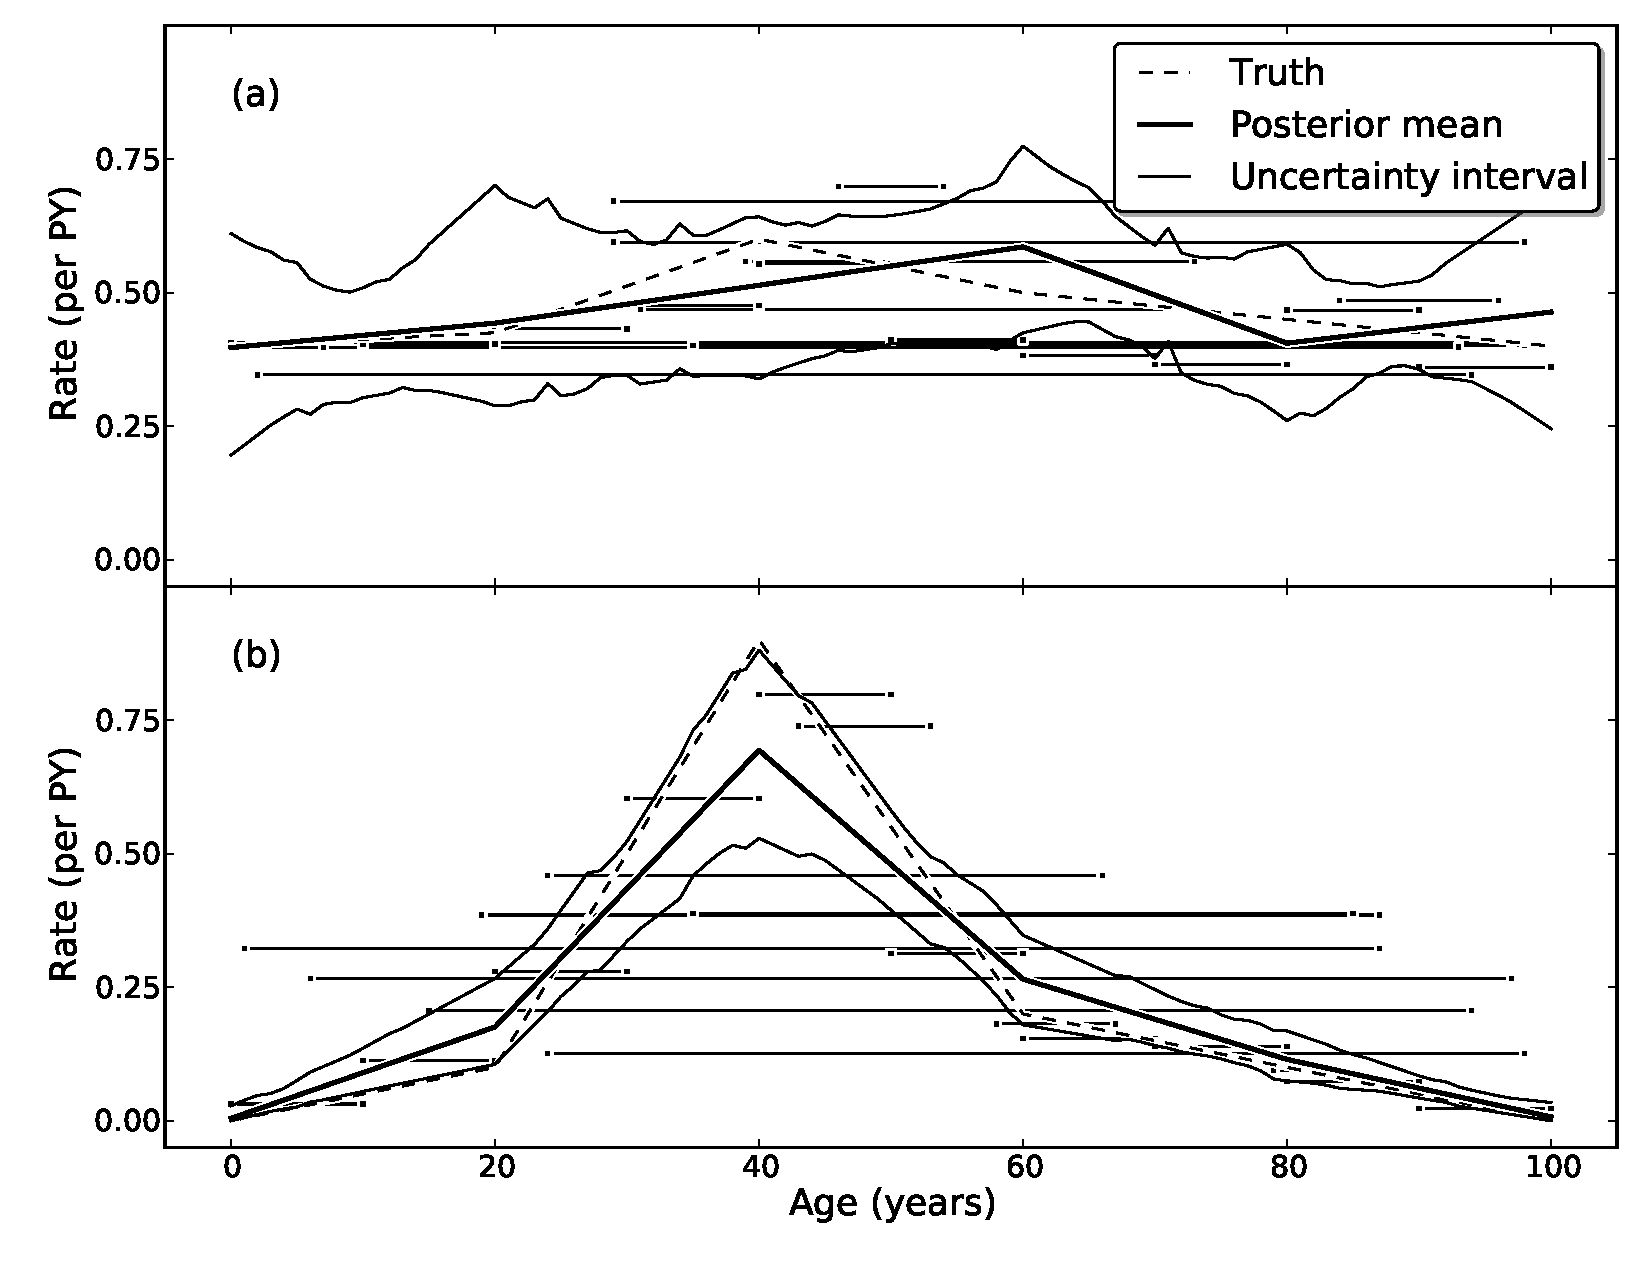
\includegraphics[width=\textwidth]{age_group_midpoint.pdf}
\caption{The midpoint model, a conceptually simple approach to
  dealing with data with heterogeneous age groups, simply
  attributes the observation to the midpoint of the age group.  Panel
  (a) shows the model applied to an age-specific hazard function that does not
  vary a great deal across ages for which the midpoint model is a
  better fit.  Panel (b) shows the model applied to an age-specific hazard function
  that varies more for which the midpoint model overcompresses the
  estimates.}
\label{midpoint}
\end{center}
\end{figure}


\section{Disaggregation model}
An alternative to the midpoint model which seems appealing but has
some downsides is what I call \emph{disaggregation}.  To understand
the disaggregation approach, imagine the simple re-analysis that I
could do if microdata were available (as described at the beginning of
this chapter).  If I had access to the individual measurements that
went into the calculation of the disease rate found in systematic
review, I could do a re-analysis with any age grouping I wished. I
could calculate rates for single-year age groups, and be sure that the
age pattern is not changing substantially during the grouping.

The microdata from rates found in systematic review are rarely
available, however. The disaggregation approach is a simple attempt to
impute what the rates for the desired age grouping would be \emph{if}
the microdata were available. This requires taking into account the
increased variation that would be found if a study of the same size
was reported for finer age groups.

Without any additional information, rate data reporting a level of $r$
for a population with effective sample size $n$ for age group $(a_s,a_e)$, i.e.,
\[
X = (r, n, a_s, a_e)
\]
can be disaggregated into $A = a_e-a_s$ rows of
data, $X_1, X_2, \ldots, X_A$, with 
\[ 
X_a = \left(r, \frac{n}{a_e-a_s}, a, a+1\right), \text{for } a=1,2,\ldots,A. 
\]

Disaggregation can be interpreted as a data preprocessing step, and
this disaggregated data can be fed to the midpoint model from the
previous section to produce a comprehensive estimate of the rate as a
function of age. However, this model has some unintended negative
features when large age intervals are disaggregated.  Because it
ignores the correlation in age of disease levels, it tends to
overcompress age patterns at young and old ages, as shown with simulated data in Figure~\ref{disagg}.

\begin{figure}[h]
\begin{center}
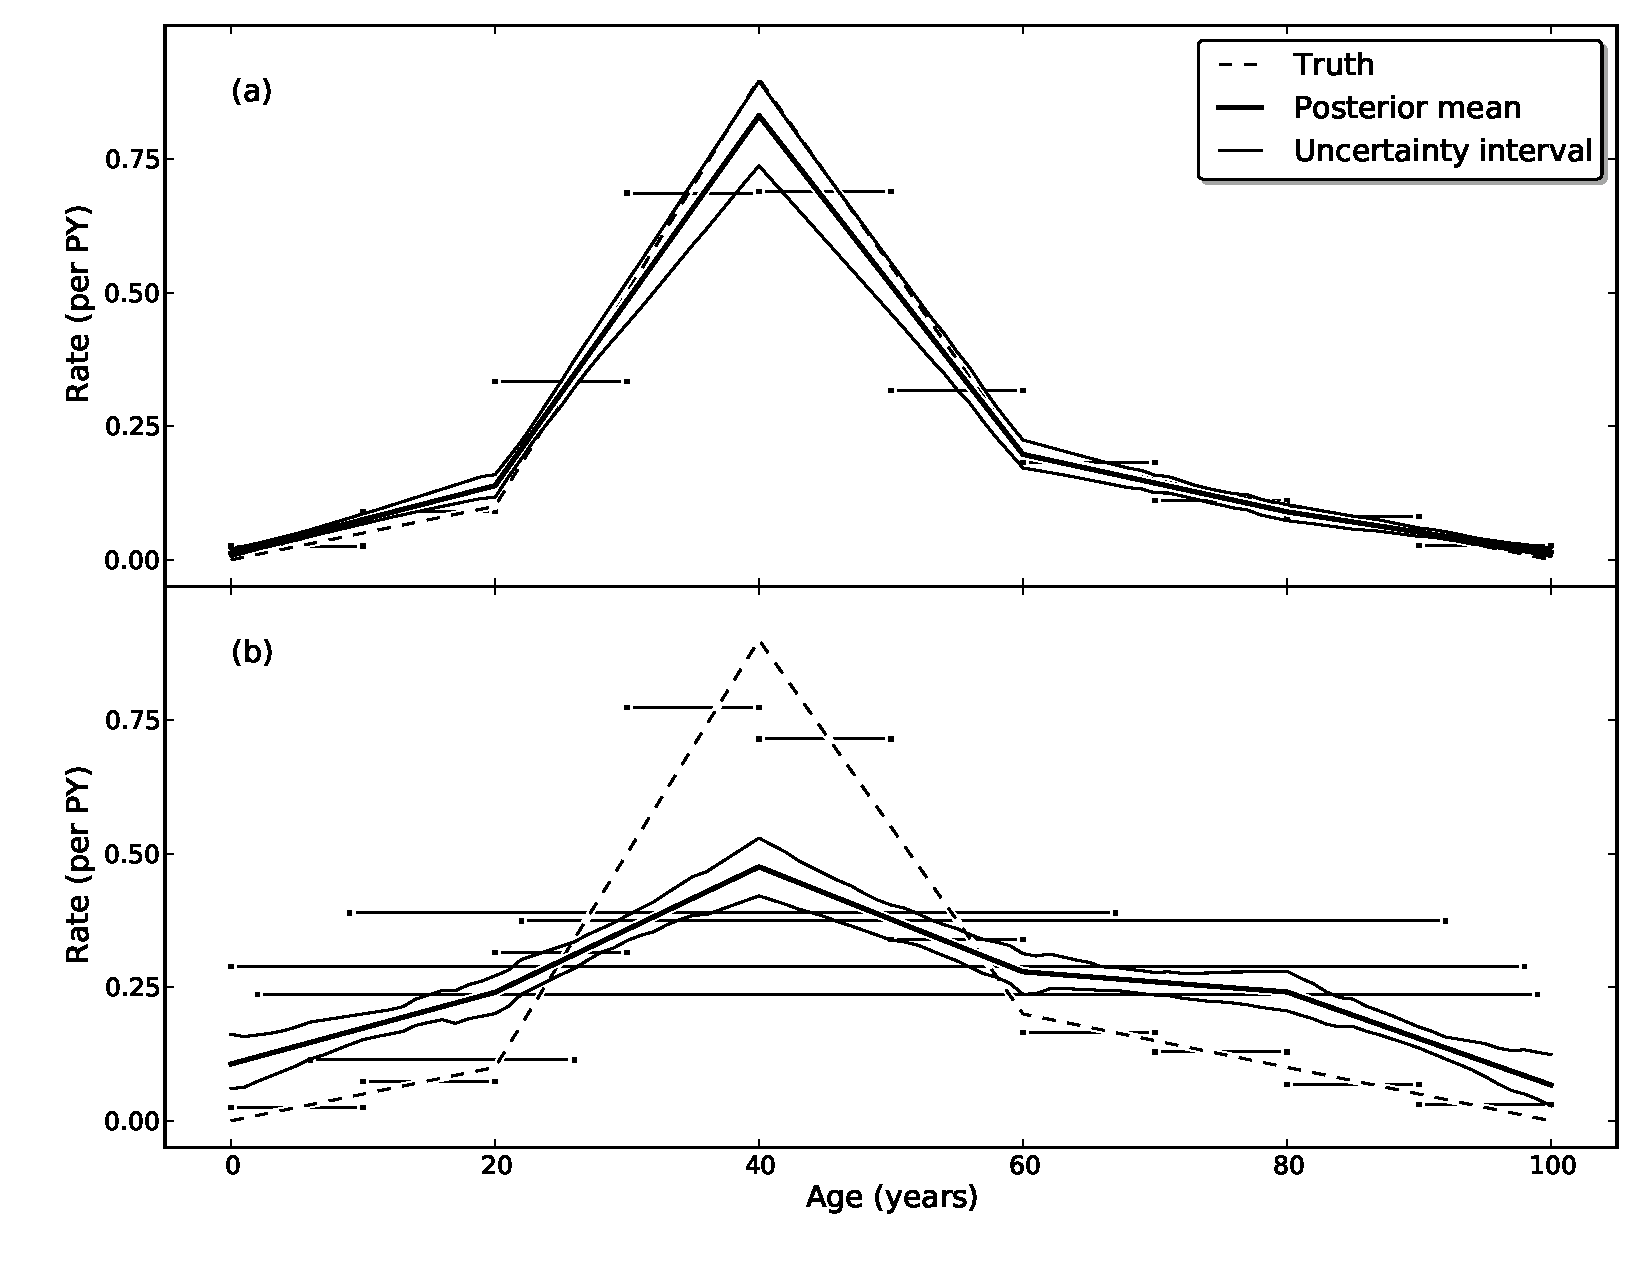
\includegraphics[width=\textwidth]{age_group_disagg.pdf}
\caption{This figure shows the effects of fitting a model with this
  disaggregation approach to two simulated data sets.  When the age groups are sufficiently
  fine-grained and homogeneous, disaggregation is a successful
  approach.  But with even slight heterogeneity, as in panel (b), the model
  estimates are overcompressed}
\label{disagg}
\end{center}
\end{figure}


\section{Midpoint model with group width covariate}
An alternative method, which I consider more ``statistical'' in its
approach, is to add the width of the age group as a covariate into the
midpoint model.  This model takes the form
\begin{align*}
r_i &\sim \scD\left(\mu_i, \rho; n_i\right),\\
\mu_i &= h\left(\frac{{a_s}_i+{a_e}_i}{2}\right) + \theta (a_e - a_s).
\end{align*}

This addresses the shortcomings of the disaggregation approach
\emph{indirectly}, and the indirect nature has positives and
negatives.  This method does not explicitly connect the large age
interval to the small age interval but instead allows the data to
inform the relationship.  On the other hand, it posits that the
data-driven relationship between the rates for studies with the same
midpoint but different age groups is a linear relationship. In
contrast, the mathematical model developed at the beginning of this
chapter is nonlinear in
a specific and mechanistically known way.
Figure~\ref{midpoint-covariate} shows the results of applying the midpoint-covariate model
model to simulated data.


\begin{figure}[h]
\begin{center}
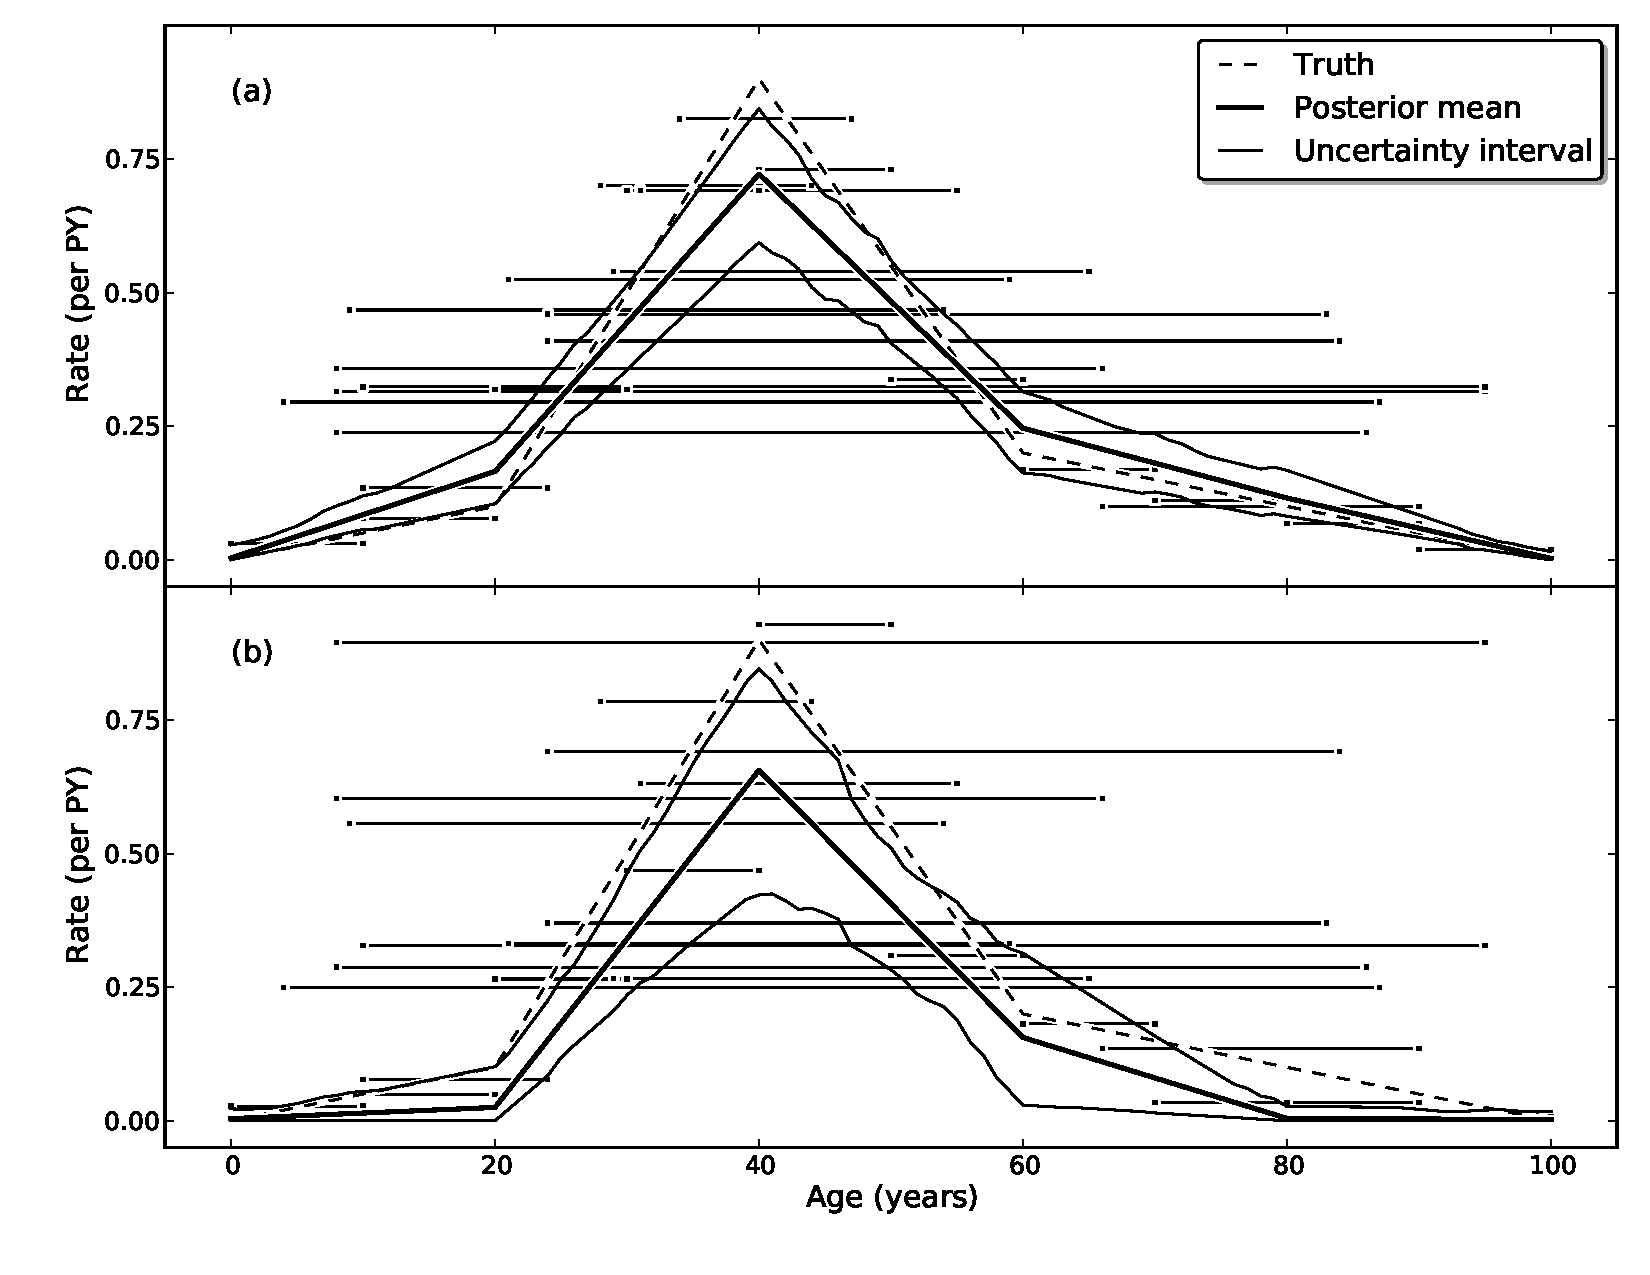
\includegraphics[width=\textwidth]{age_group_midpoint_covariate.pdf}
\caption{The midpoint-covariate model applied to two simulated
  datasets, where ground truth is known. Although this approach is
  appealing theoretically, the added flexibility of the covariate
  model does not add much value in the simulation study. }
\label{midpoint-covariate}
\end{center}
\end{figure}

\section{Age-standardizing and age-averaging models}
An even more complicated approach, both conceptually and
computationally, is to average across the age interval explicitly in
the statistical model:
\begin{align*}
r_i &\sim \scD\left(\mu_i, \rho; n_i\right),\\
\mu_i &= \int_{a={a_s}_i}^{{a_e}_i} h(a)\d w_i(a),
\end{align*}
where the integration $\d w_i$ is weighted according to population
structure.

This has the theoretical appeal of matching the generative model above
but the drawback of being slower to compute and less stable
numerically.  It also has a major piece left unspecified, the
selection of the age weights for the integration.  There are two
sensible approaches to this, which I call the \emph{age-standardizing
  model} and the \emph{age-averaging model}.  The age-standardizing
model uses a common age pattern $\d w_i(a) = \d w(a)$ for all studies, while
the age-averaging model uses the best estimate available of the age
pattern of the study population in each observation.  The
age-standardizing model is faster, due to a computational optimization
only possible when the $\d w_i$ are the same for all $i$, but the
age-averaging model is appealing on theoretical grounds, because it
can make use the most information.  However, it is not certain that
using this information will make the end results any more accurate,
because the age pattern of the study population is rarely known with
much certainty, and often it is necessary to assume that it matches
the national age pattern for the country-years where the study was
conducted.  In the case of remission and mortality studies it is even
more complicated to estimate the study population age pattern, since
it is \emph{not} the same as the national population age pattern, but
modulated by the age pattern of disease prevalence.
Figure~\ref{age-group-standardize} shows the results of this model on
simulated data.

\begin{figure}[h]
\begin{center}
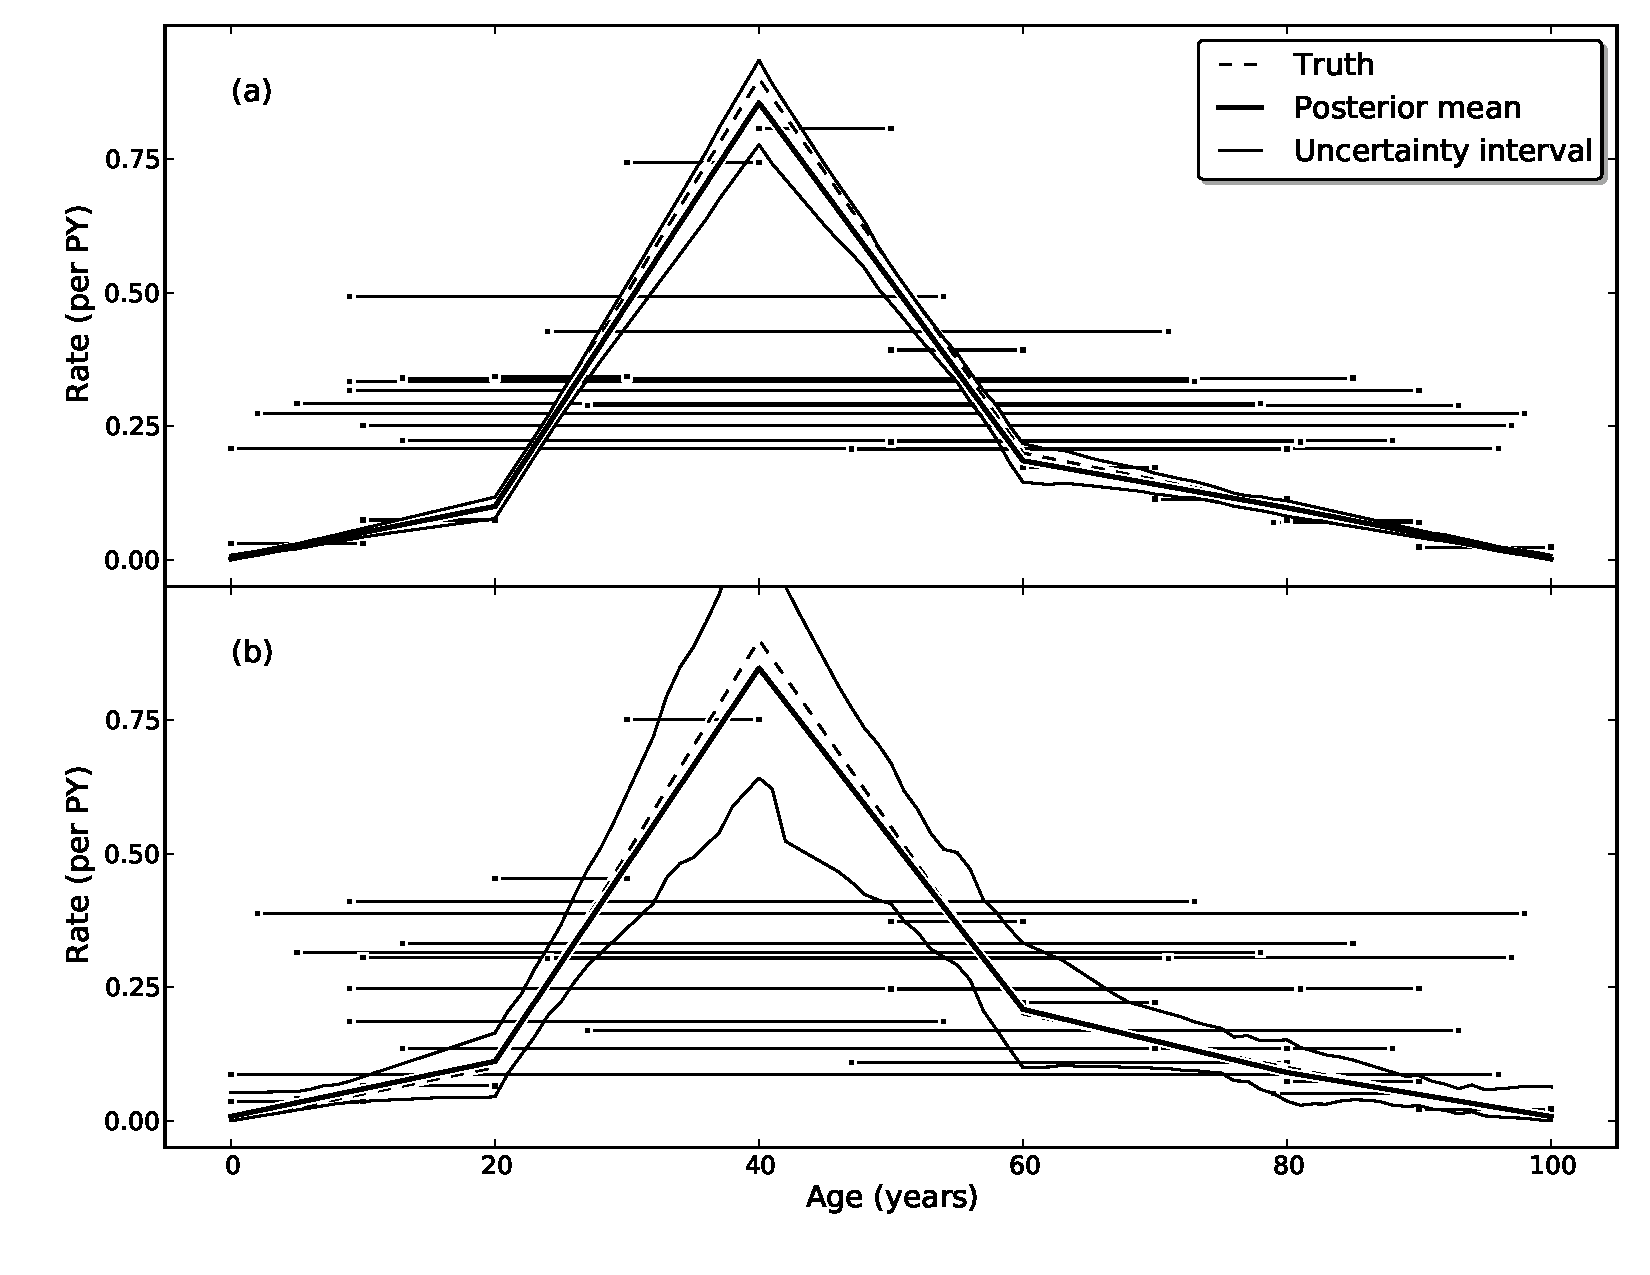
\includegraphics[width=\textwidth]{age_group_standardize.pdf}
\caption{The age-standardizing model applied to simulated data with a
  known age-specific rate function as ground truth.  The results in
  panel (a) show that the model 
  recovers the true age pattern quite precisely. Panel (b) shows that the
  results are still accurate when the data generation procedure is
  even more noisy.}
\label{age-group-standardize}
\end{center}
\end{figure}


\section{Model comparison}
\label{agm-compare}

\begin{figure}[h]
\begin{center}
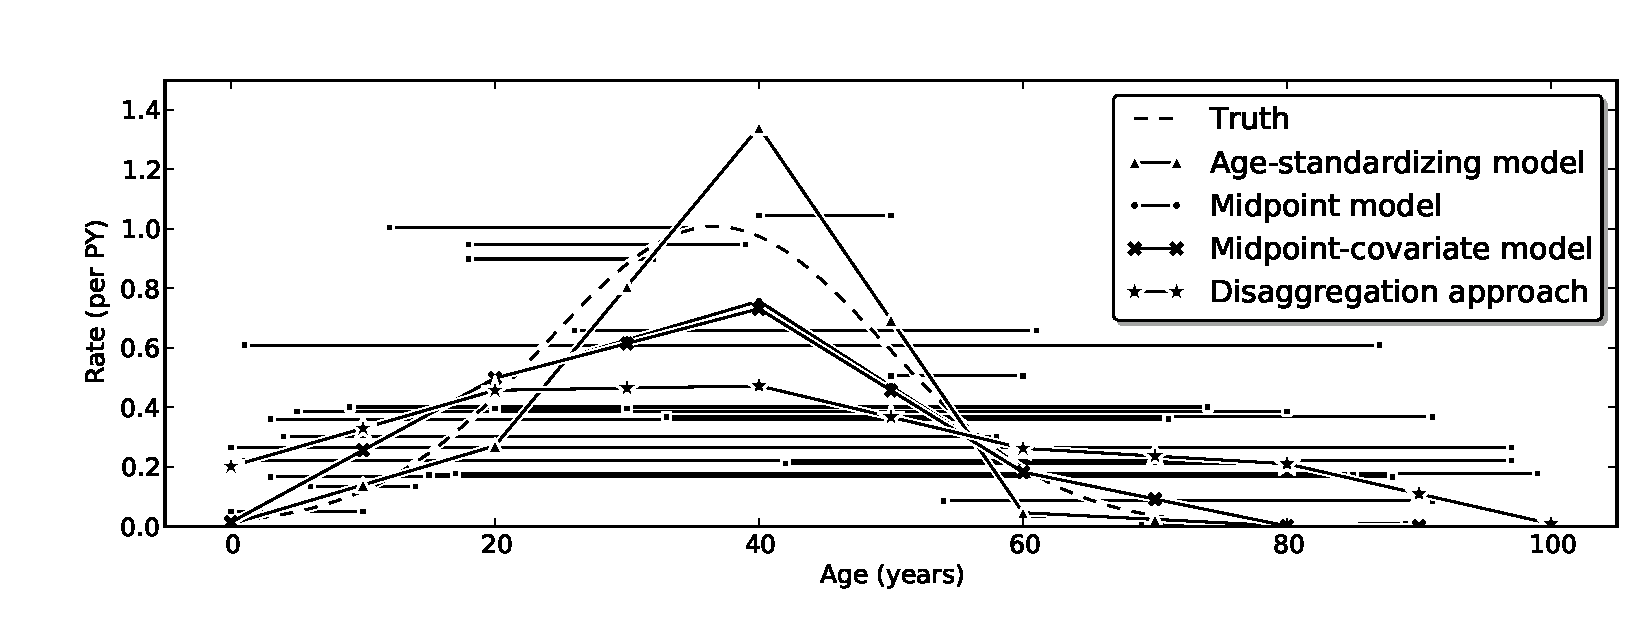
\includegraphics[width=\textwidth]{age_group_models.pdf}
\caption{A comparison of $4$ models for heterogeneous age groups, showing that the age-standardizing model comes closest to recovering the truth.  This corresponds to the results of the simulation study presented below in Table~\ref{age_group_comparison}.}
\label{age-group-model-comparison}
\end{center}
\end{figure}


This section provides a comparison of the approaches to age group
modeling.

An appropriate comparison of these approaches is somewhat difficult to
develop.  One approach is through simulation study, where a dataset is
simulated from known ground truth.  This allows the estimates to be
compared to ``true'' values, but this risks
inappropriate model selection due to inaccurately choosing the
distribution of the simulated data.  Another approach is
cross-validation, where data from systematic review is split into
mutually exculsive
\emph{training} and \emph{test} sets, and the model is fit to the
training set and used to predict the values in the test set.  Naively
holding out $25\%$ of the data doesn't address the exact topic of
interest, however, since it determines which model predicts rates of
all age groups, and I am really only interested in predicting the age
groups with small widths accurately.  It would be preferable to hold
out only data with small-width age groups from large representative
subpopulations.  Unfortunately there is rarely enough data to do this,
especially in all the settings that come up in disease modeling.

I have taken a pragmatic approach, evaluating with a natural
simulation described below.  Future work, based on more sophisticated
simulation scenarios or based on carefully designed hold-out
cross-validation, is necessary to further understand the trade-offs
between these alternative methods.

The data simulation procedure I used is the following:
\begin{itemize}
\item Choose age intervals for $30$ rows of data; for $i=1,\ldots,10$,
  $({a_s}_i,{a_e}_i) = (10(i-1), 10i)$, and for the remaining $20$
  intervals, choose the age interval width uniformly at random from $[1,100]$
  and choose the midpoint of the age interval uniformly at random from ages
  which admit this age range.

\item Choose the effective sample size $n_i$ for each row, uniformly at random from $[10^2, 10^4]$.

\item Choose an age-specific population structure for each row of data,
  with the form $w_i(a) = e^{\beta_i a}$, where $\beta_i$ is drawn
  from a normal distribution with mean $0$ and standard deviation
  $\frac{1}{10}$.

\item Calculate the true rate value for each age interval,
  $r^\text{true}_i = \sum_{a={a_s}_i}^{{a_e}_i} \mu_\text{true}(a)
  w_i(a)$, where $\mu_\text{true}(a) =
  \exp\left(\frac{3(a-35)^2}{1000} + \frac{a-35}{100}\right).$

\item Choose an observed rate value, based on a negative binomial distribution:
$r_in_i \sim \NegativeBinomial(r^\text{true}_i, \delta_\text{true})$, where $\delta_\text{true} = 5$.
\end{itemize}

Table~\ref{age_group_comparison} shows the median results of fitting this simulated data with a variety of models.

\begin{table}

\begin{center}
\begin{tabular}{|c|c|c|c|c|}
\hline
model&bias&mae&pc&time\\
\hline
midpoint&0.02&0.08&0.8&29.0\\
disaggregation&0.03&0.19&0.08&52.6\\
midpoint-covariate&0.03&0.09&0.89&45.8\\
age-standardizing&0.01&0.04&0.95&30.3\\
age-integrating&-0.0&0.03&0.78&38.1\\
\hline
\end{tabular}
\end{center}

\caption{Median results for $100$ replicates of the simulation study
  comparing age-specific rate estimates from $5$ models of age-grouped
  data, showing bias (mean of true minus predicted), median absolute
  error (mae, median of absolute difference between truth and
  predicted), probability coverage (pc, fraction of truth falling
  within 95\% uncertainty interval of prediction), and computation time. The
  age-standardizing and age-integrating models are superior in all
  metrics of fit quality.  The age-standardizing model has computation time only slightly more
  than the fastest approach, while the age-integrating model is 26\% slower.}
\label{age_group_comparison}
\end{table}


\bibliographystyle{plain}
\bibliography{my_library}
\end{document}
